\documentclass{templateNote}

\definecolor{Verde}{RGB}{170,239,31}
\definecolor{Morado}{RGB}{127,0,255}
\definecolor{Celeste}{RGB}{0,191,255}
\definecolor{Salmon}{RGB}{255,0,157}
\definecolor{RosaSuave}{RGB}{255,182,193}
\definecolor{Melocoton}{RGB}{255,218,185}
\definecolor{Gris}{RGB}{192,192,192}
\definecolor{Turquesa}{RGB}{64,224,208}
\definecolor{Menta}{RGB}{152,251,152}
\definecolor{AmarilloVainilla}{RGB}{255,255,153}

\newcommand{\newparagraph}{\par\vspace{\baselineskip}\noindent}
\newcommand{\hlcolor}[2]{{\sethlcolor{#1}\hl{#2}}}

\begin{document}

\imagenlogoU{img/LogoElNube.png}
\linklogoU{https://github.com/MarceloPazPezo}
\linkQRDoc{https://github.com/MarceloPazPezo/MyRepo/tree/main/Icinf}
\titulo{Guia de ejercicios: Certamen 2}
\asignatura{Administración y Programación de Base de Datos}
\autor{
Marcelo Paz
}
\vDoc{1.0.0}
\tipoDoc{Apunte}

% Metadatos del PDF
\title{[\asignatura]-\titulo}
\author{
    \autor
}
\portada
\margenes % Crear márgenes

\section{Sección de prueba}
\begin{enumerate}
    \item Traspasar la consulta SQL a un árbol de consulta.
    \begin{tcolorbox}[
        colback=Verde!30,
        colframe=Verde!90!black]
        \begin{verbatim}
SELECT apellido1
FROM Empleado E, TrabajaEn T, Proyecto P
WHERE nameProy = 'Aquarius' 
AND T.idProy = P.idProy
AND E.idEmpleado = T.idEmpleado
AND E.FechaNacimiento > '21-12-1957';
        \end{verbatim}
    \end{tcolorbox}
    \begin{enumerate}
        \item Obtener el árbol inicial (canónico) de la consulta.
        \begin{figure}[H]
            \centering
            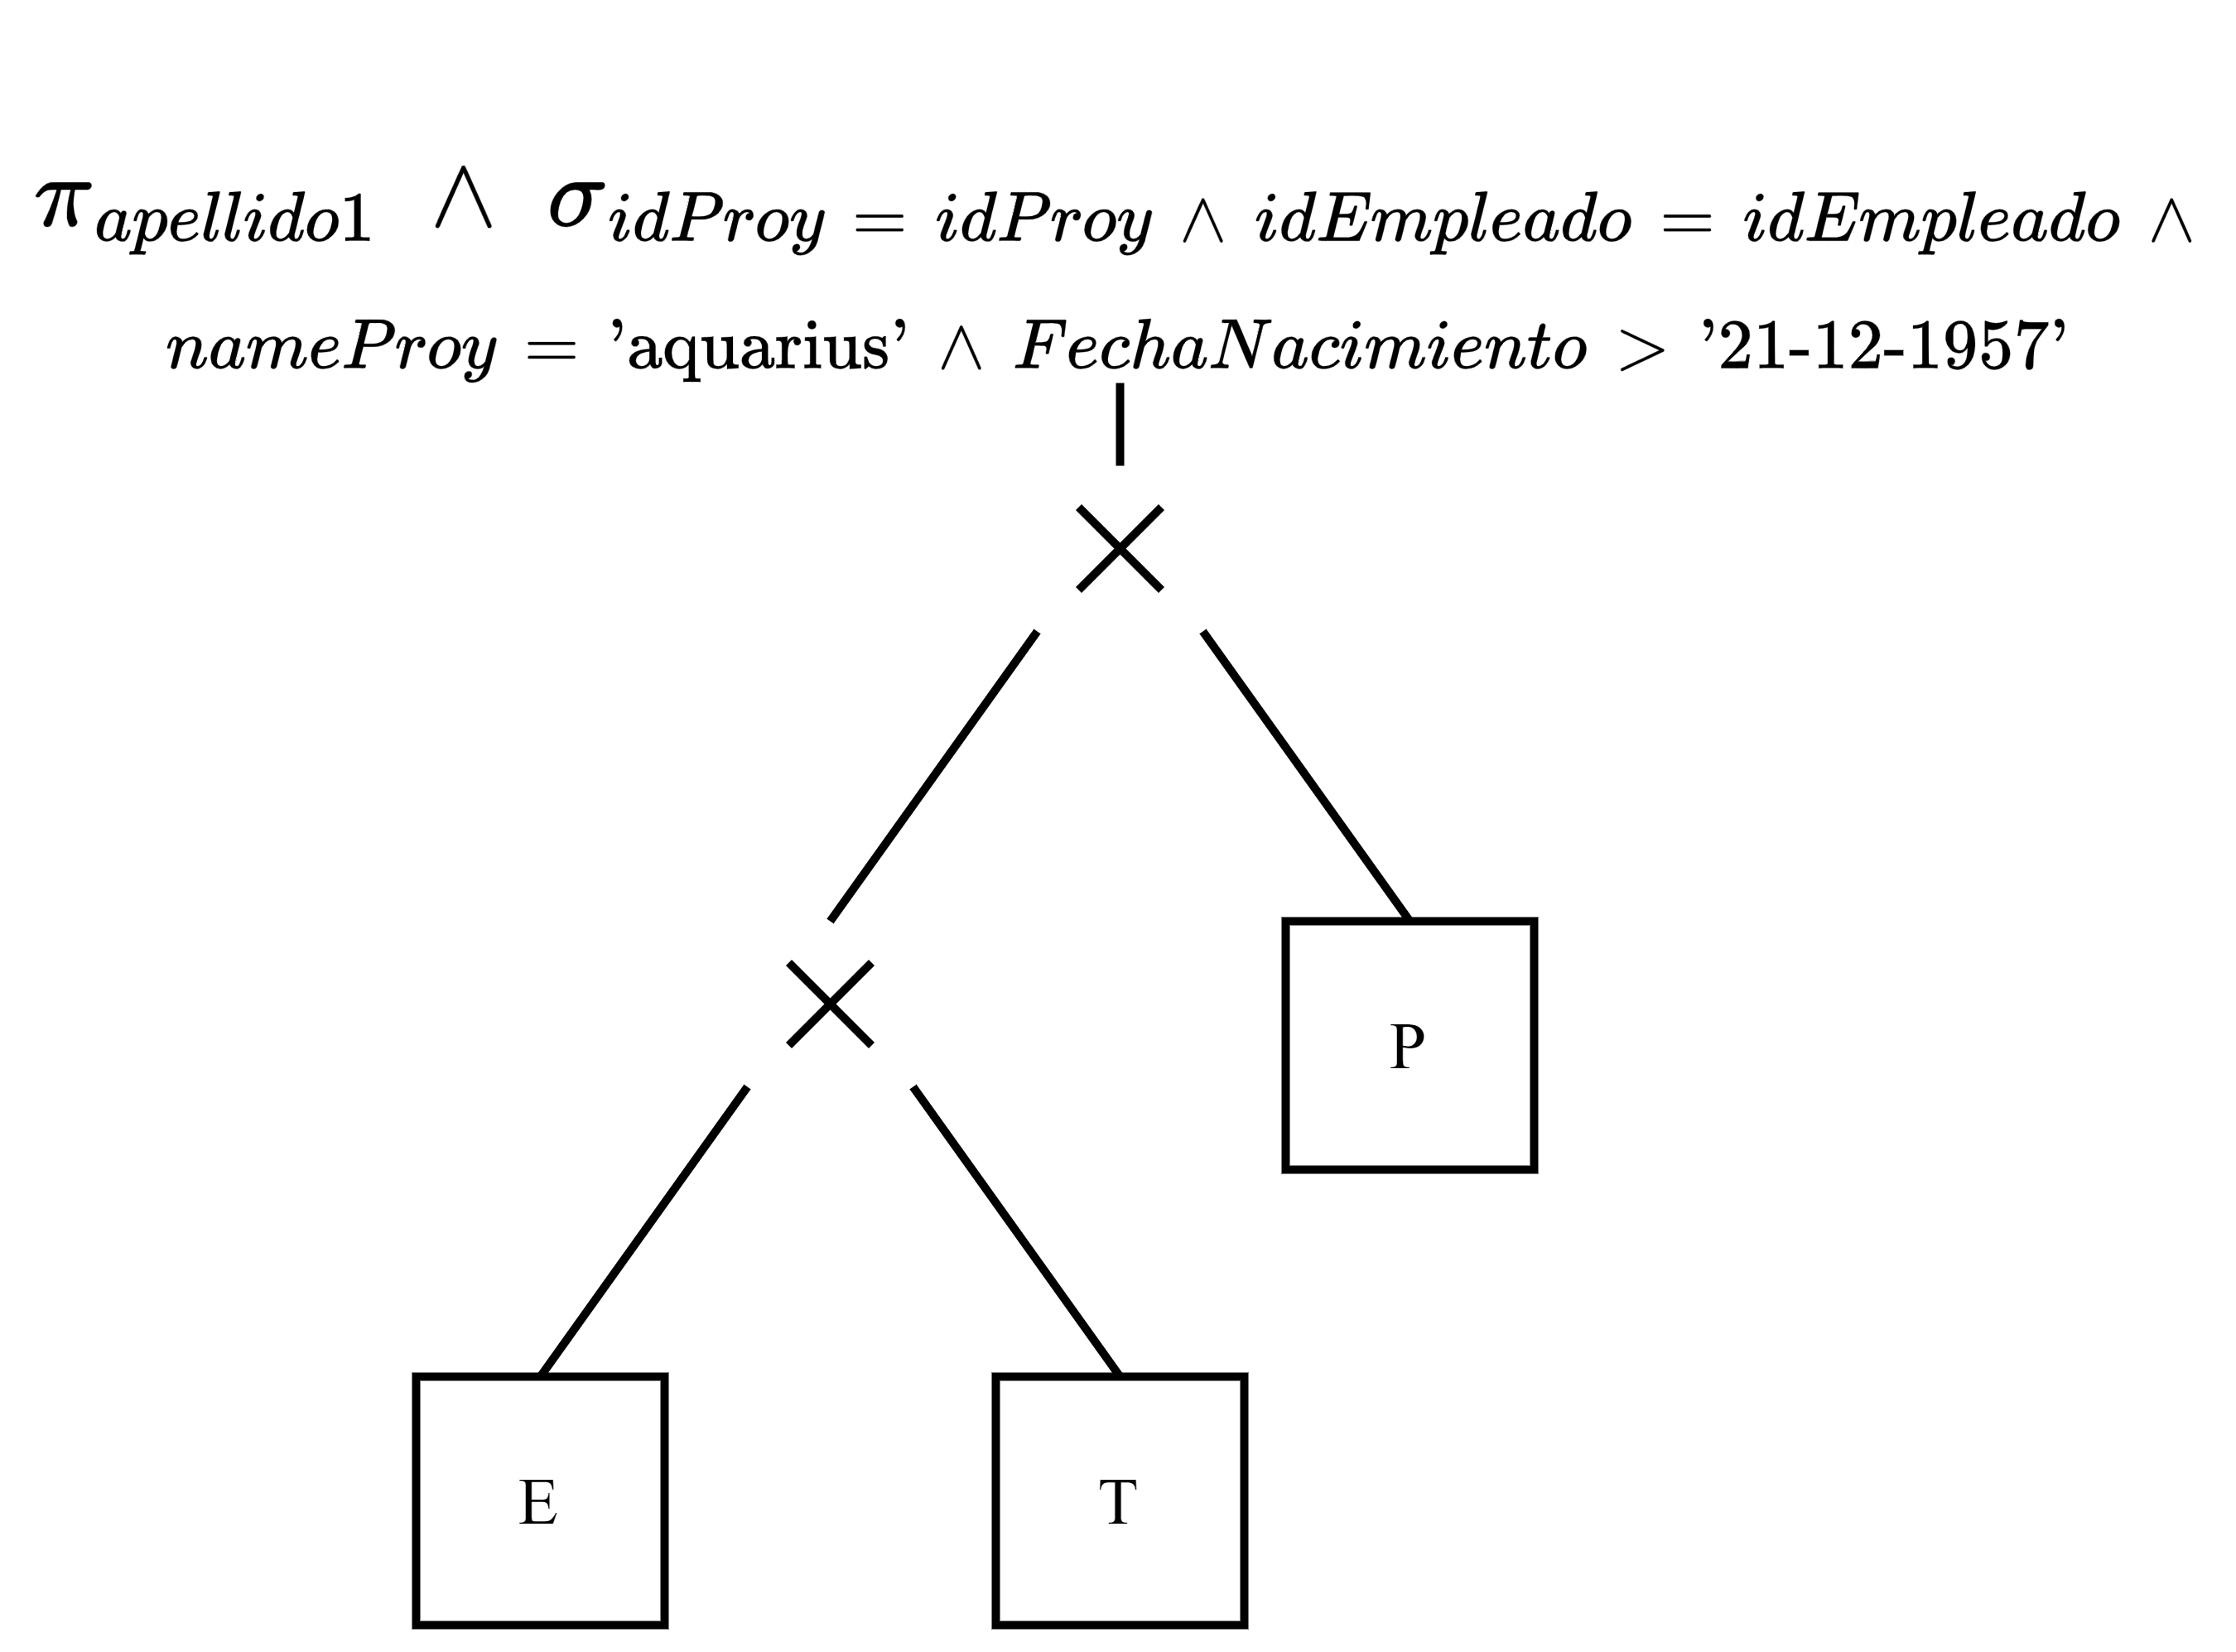
\includegraphics[width=0.8\textwidth]{img/E1-ArbolCanonico.png}
        \end{figure}

        \newpage
        \item Explique como se optimiza el árbol de consulta mediante la optimización vista en clases.
        \begin{enumerate}
            \item Se separa la proyección y las selecciones por tablas.
            \begin{figure}[H]
                \centering
                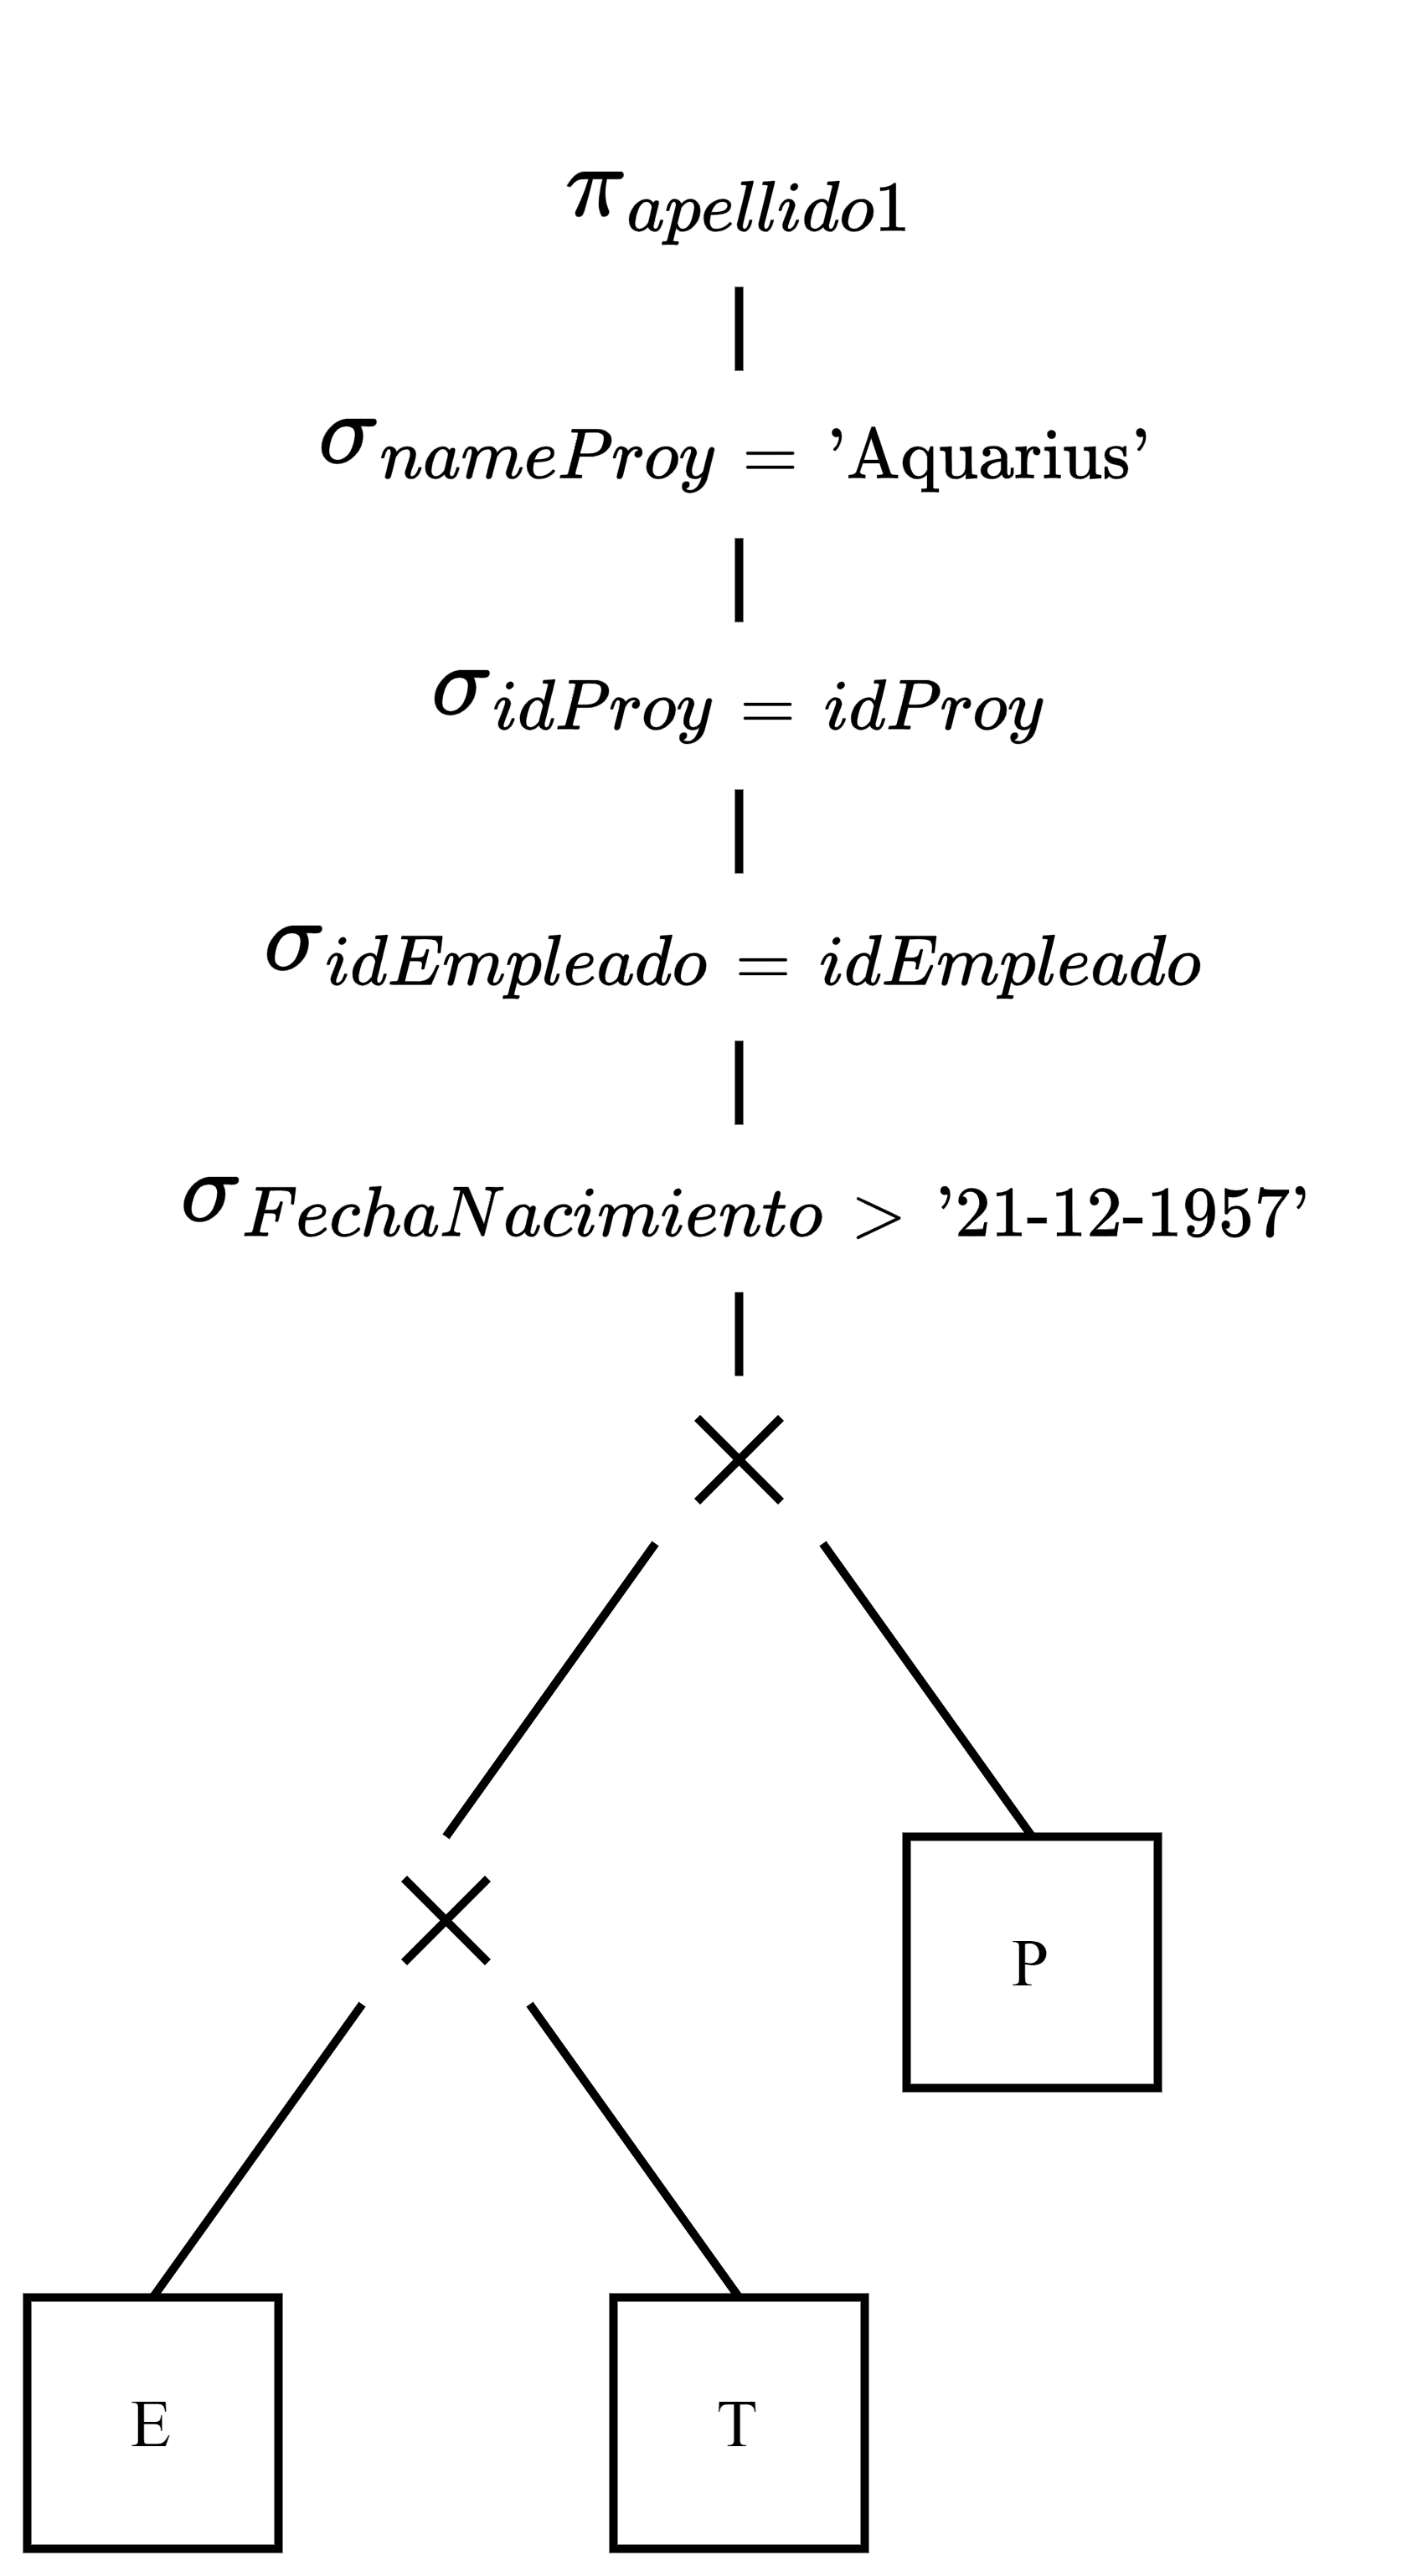
\includegraphics[width=0.45\textwidth]{img/E1-Paso1.png}
            \end{figure}

            \newpage
            \item Se reorganizan las tablas buscando la forma más optimas de unir las tablas (Solo si es posible).
            \begin{figure}[H]
                \centering
                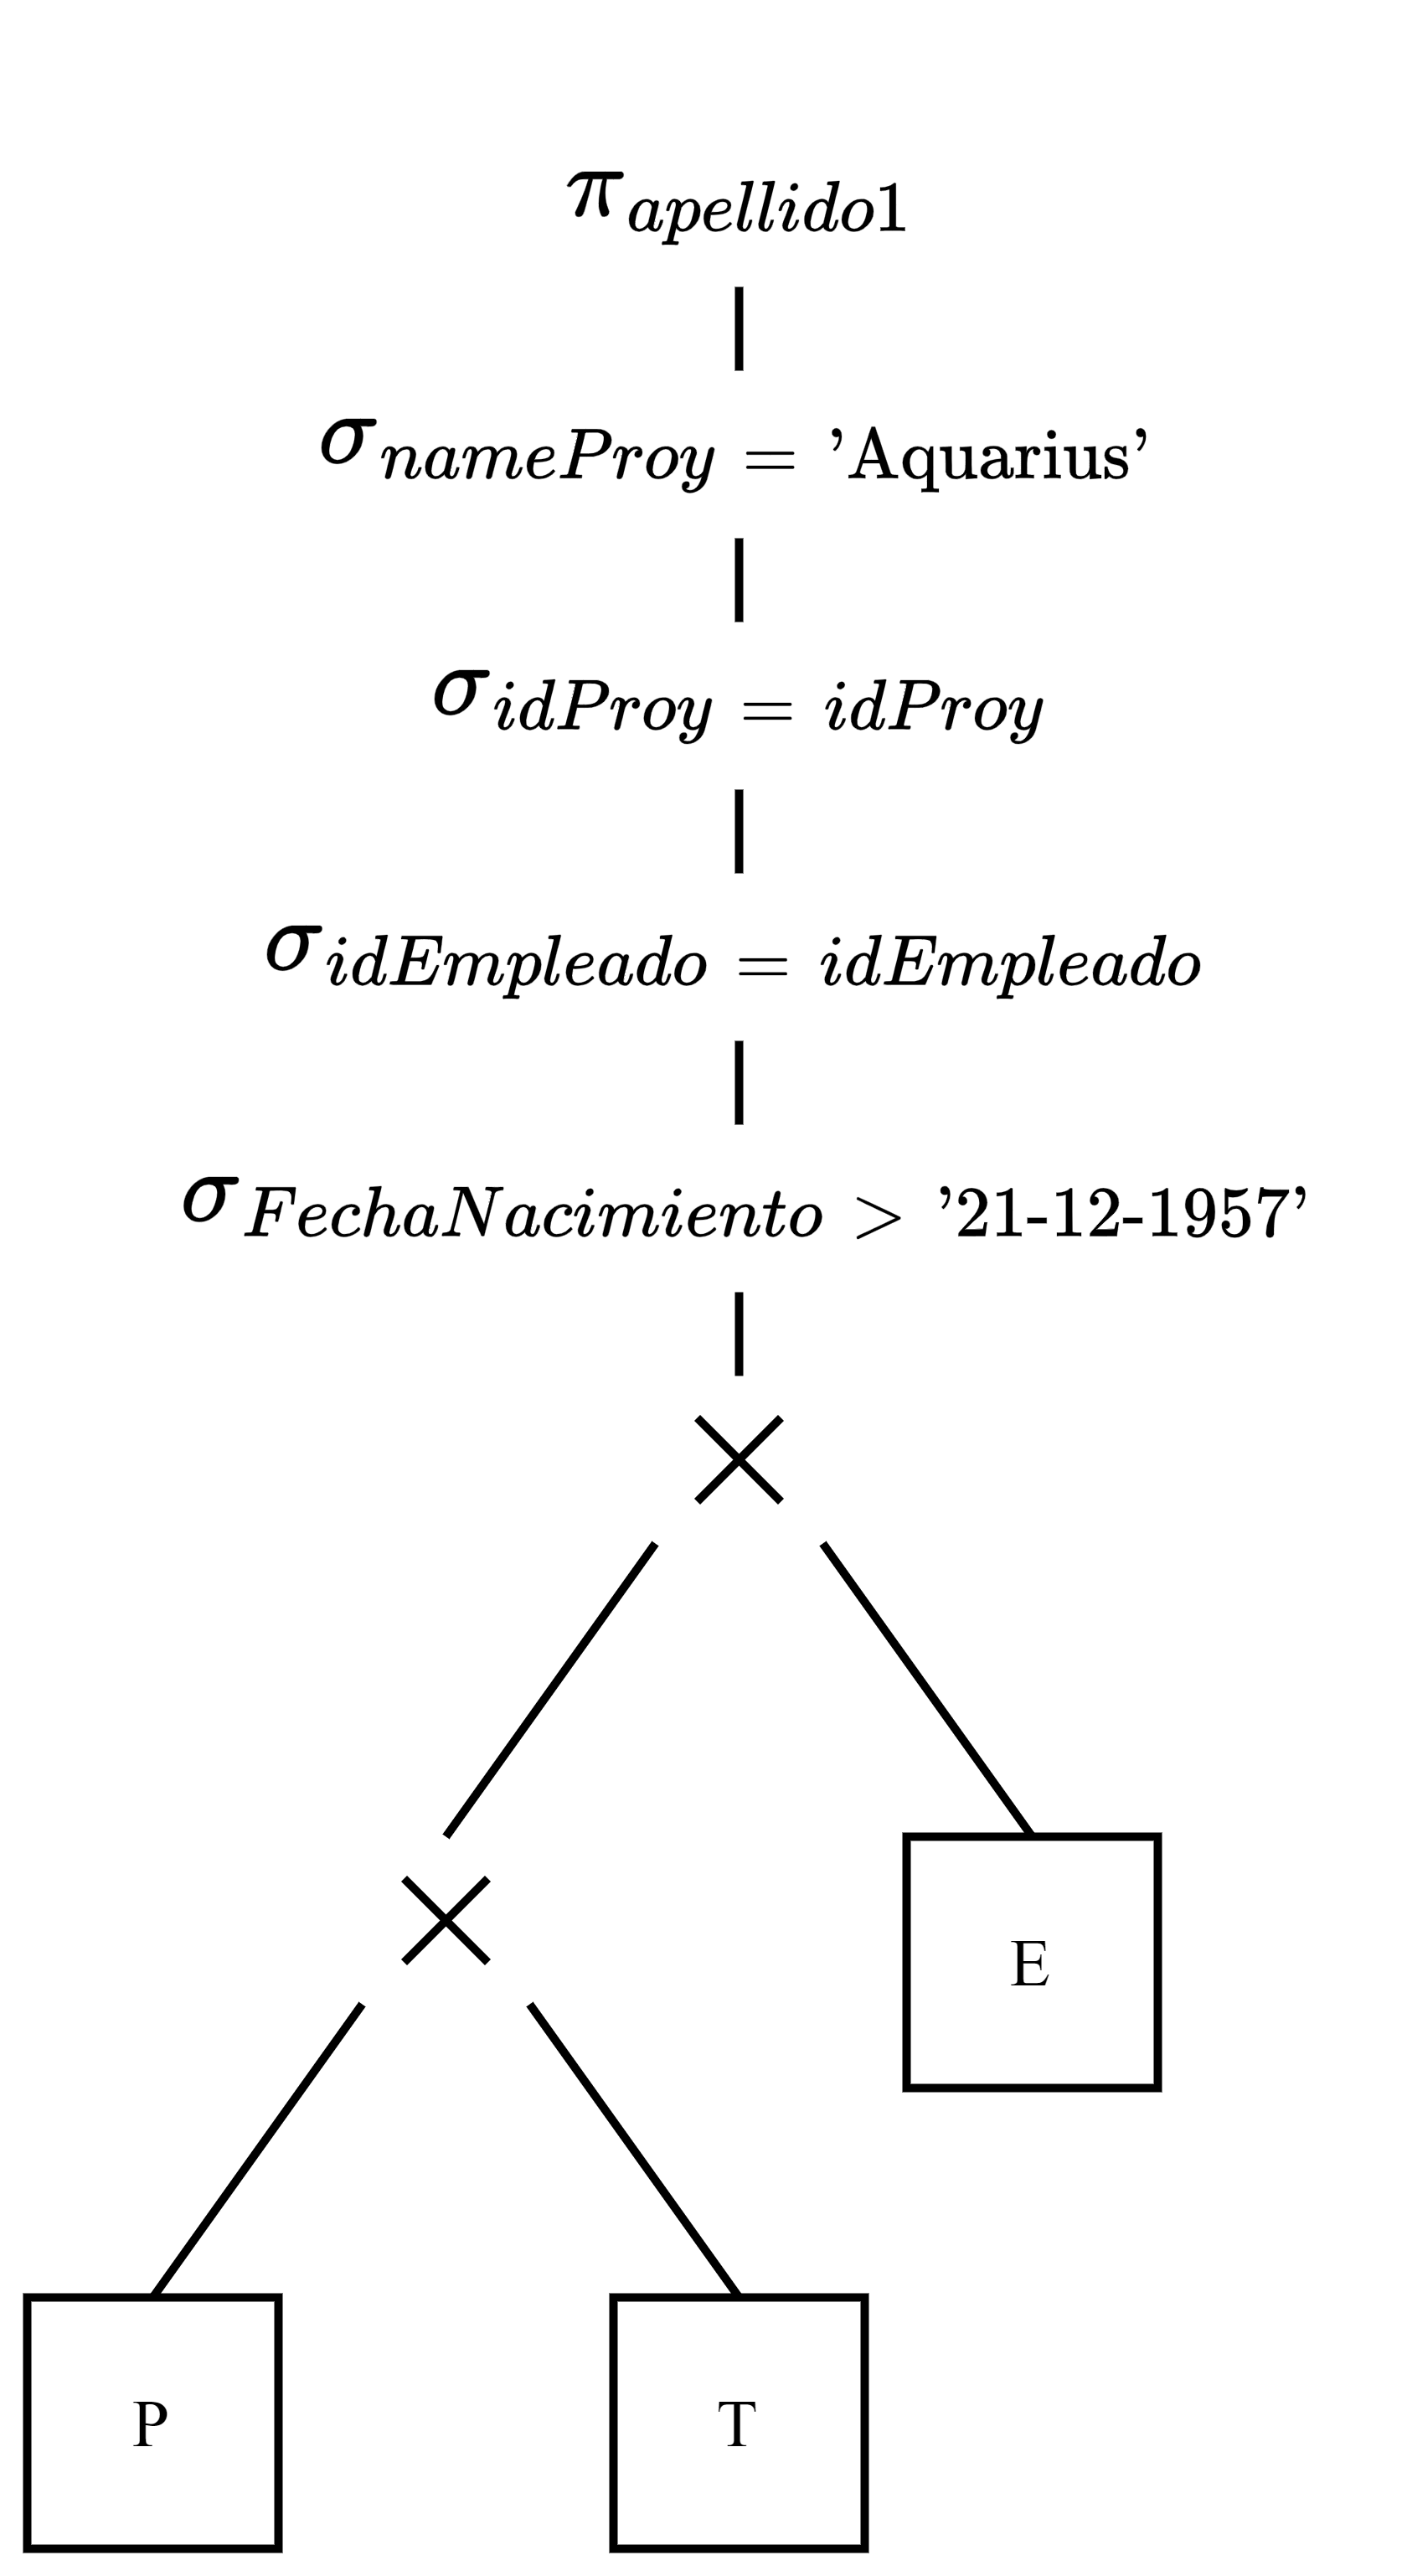
\includegraphics[width=0.35\textwidth]{img/E1-Paso2.png}
            \end{figure}

            \item Se bajan las selecciones hasta su respectivo producto cartesiano.
            \begin{figure}[H]
                \centering
                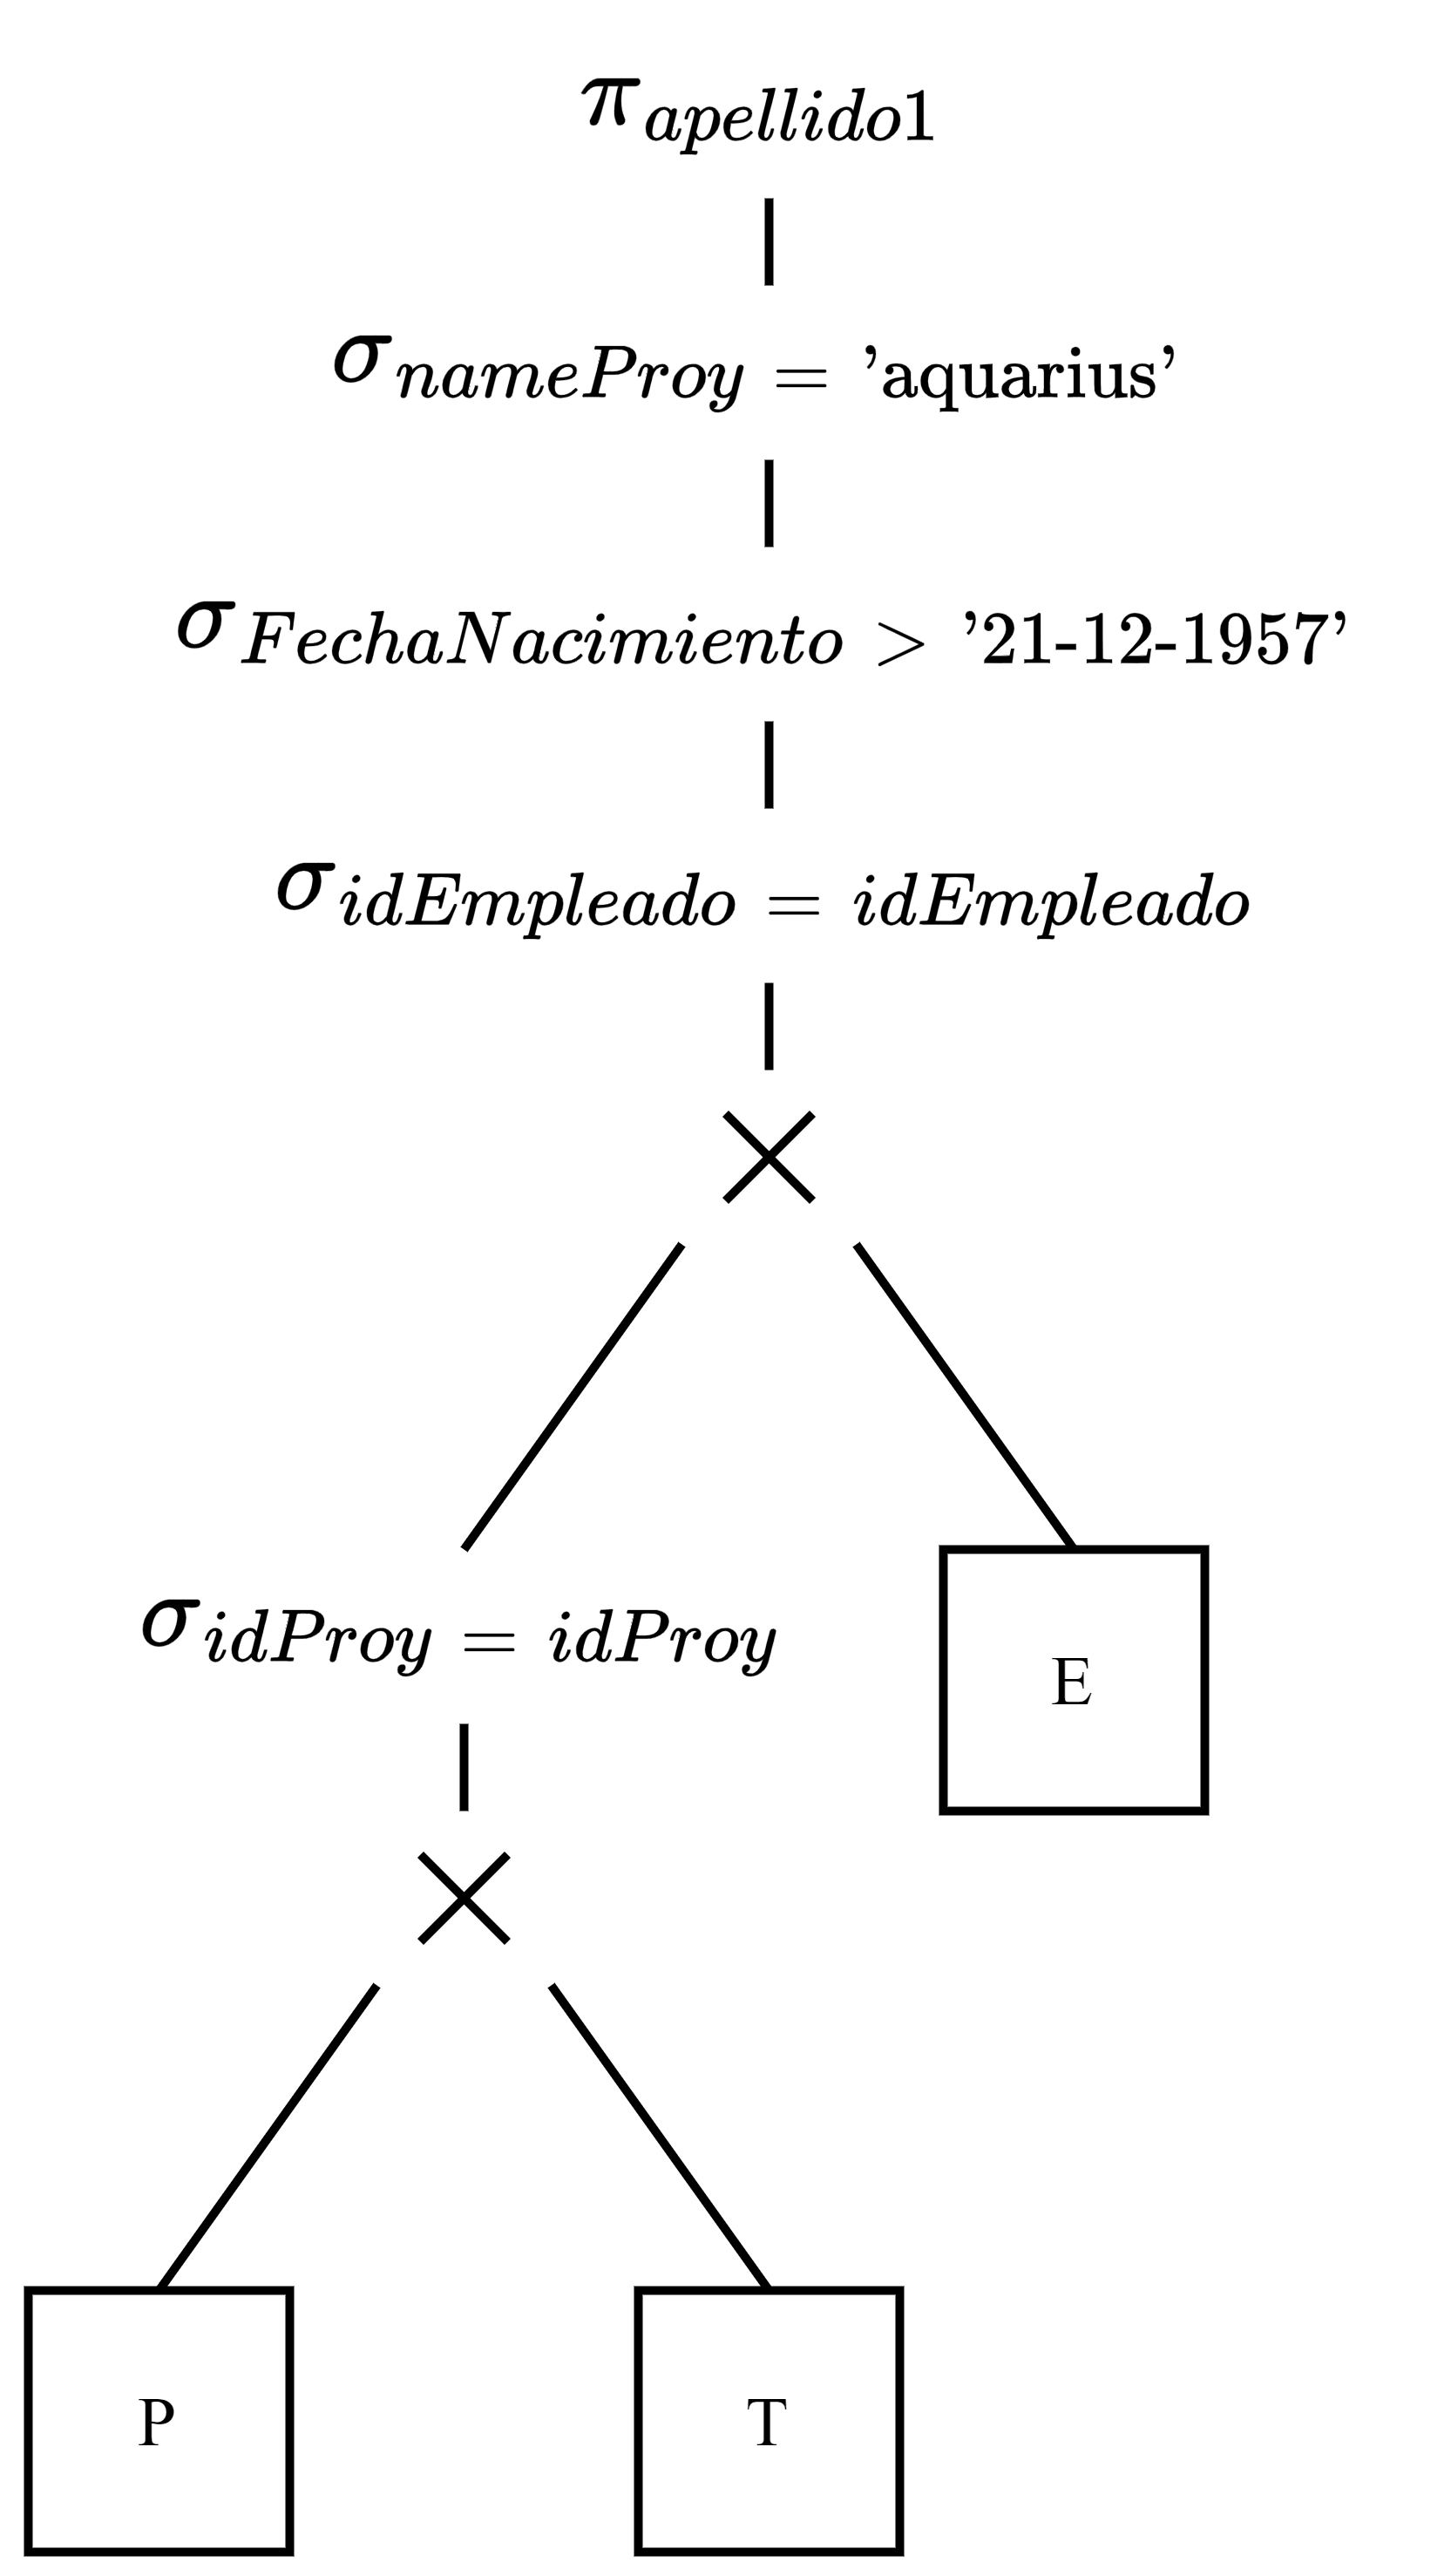
\includegraphics[width=0.35\textwidth]{img/E1-Paso3.png}
            \end{figure}

            \newpage
            \item Se cambia la seleccion y el producto cartesiano por un join.
            \begin{figure}[H]
                \centering
                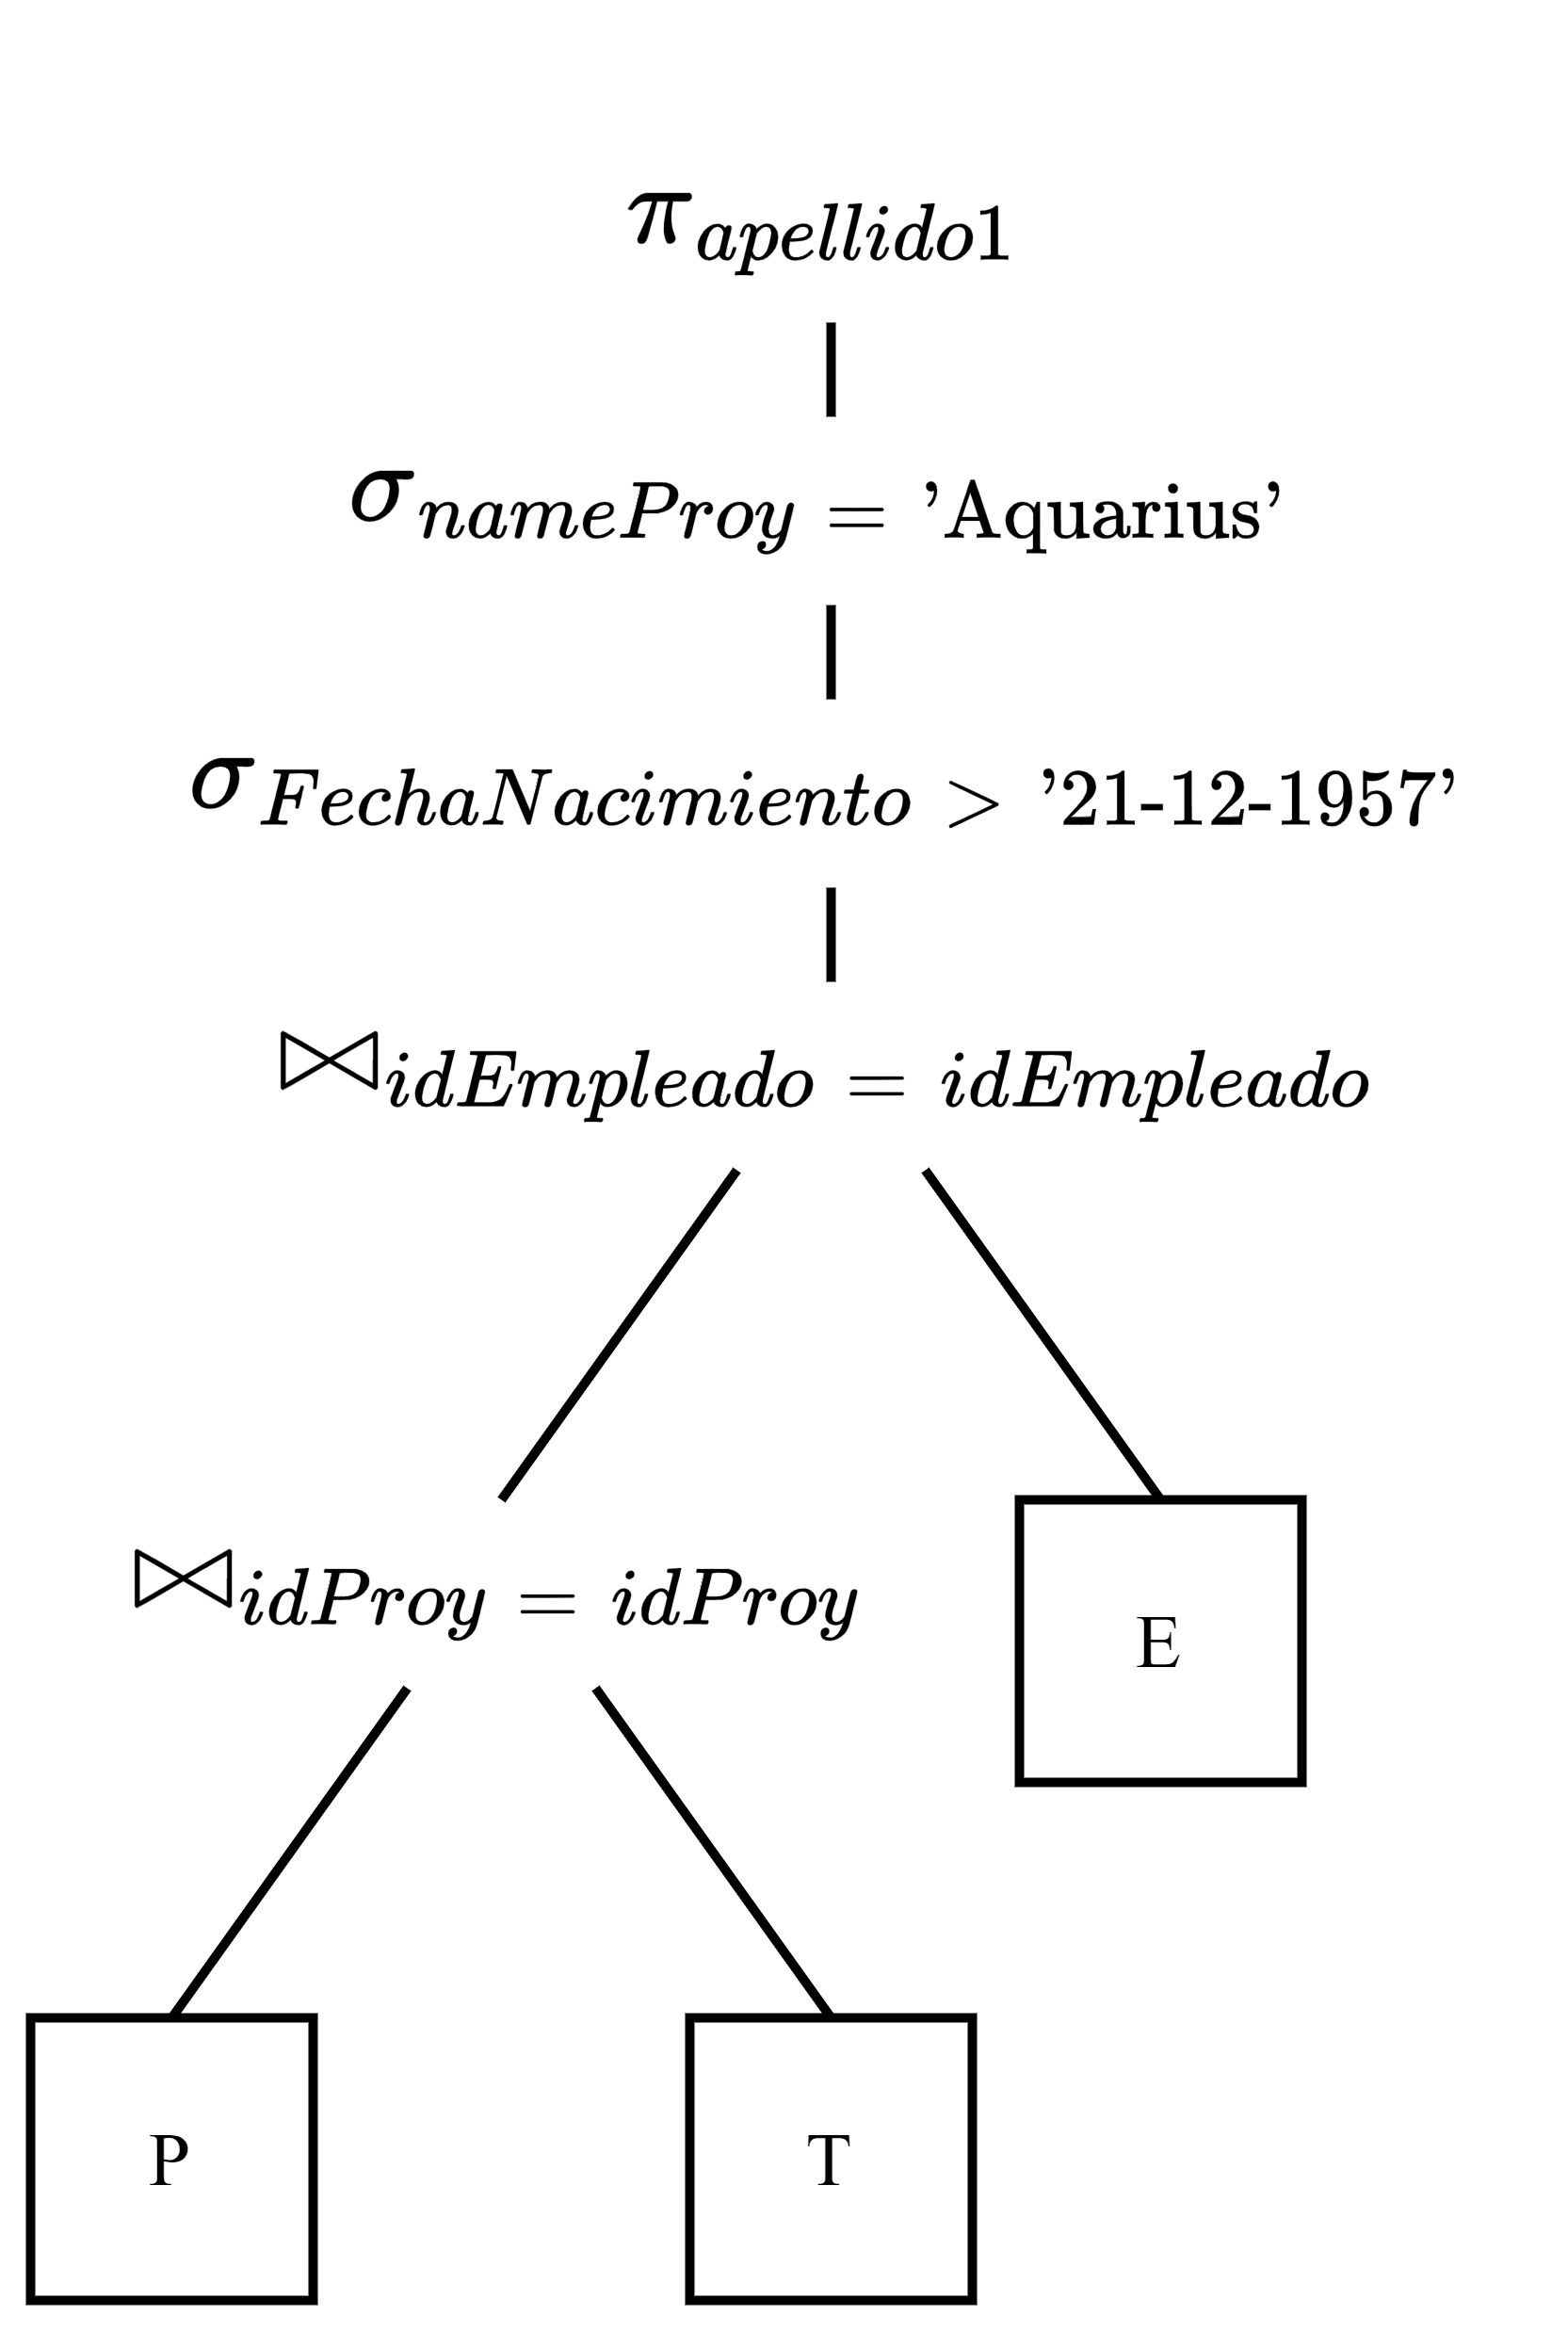
\includegraphics[width=0.4\textwidth]{img/E1-Paso4.png}
            \end{figure}

            \item Se bajan las demas selecciones a sus respectivas tablas.
            \begin{figure}[H]
                \centering
                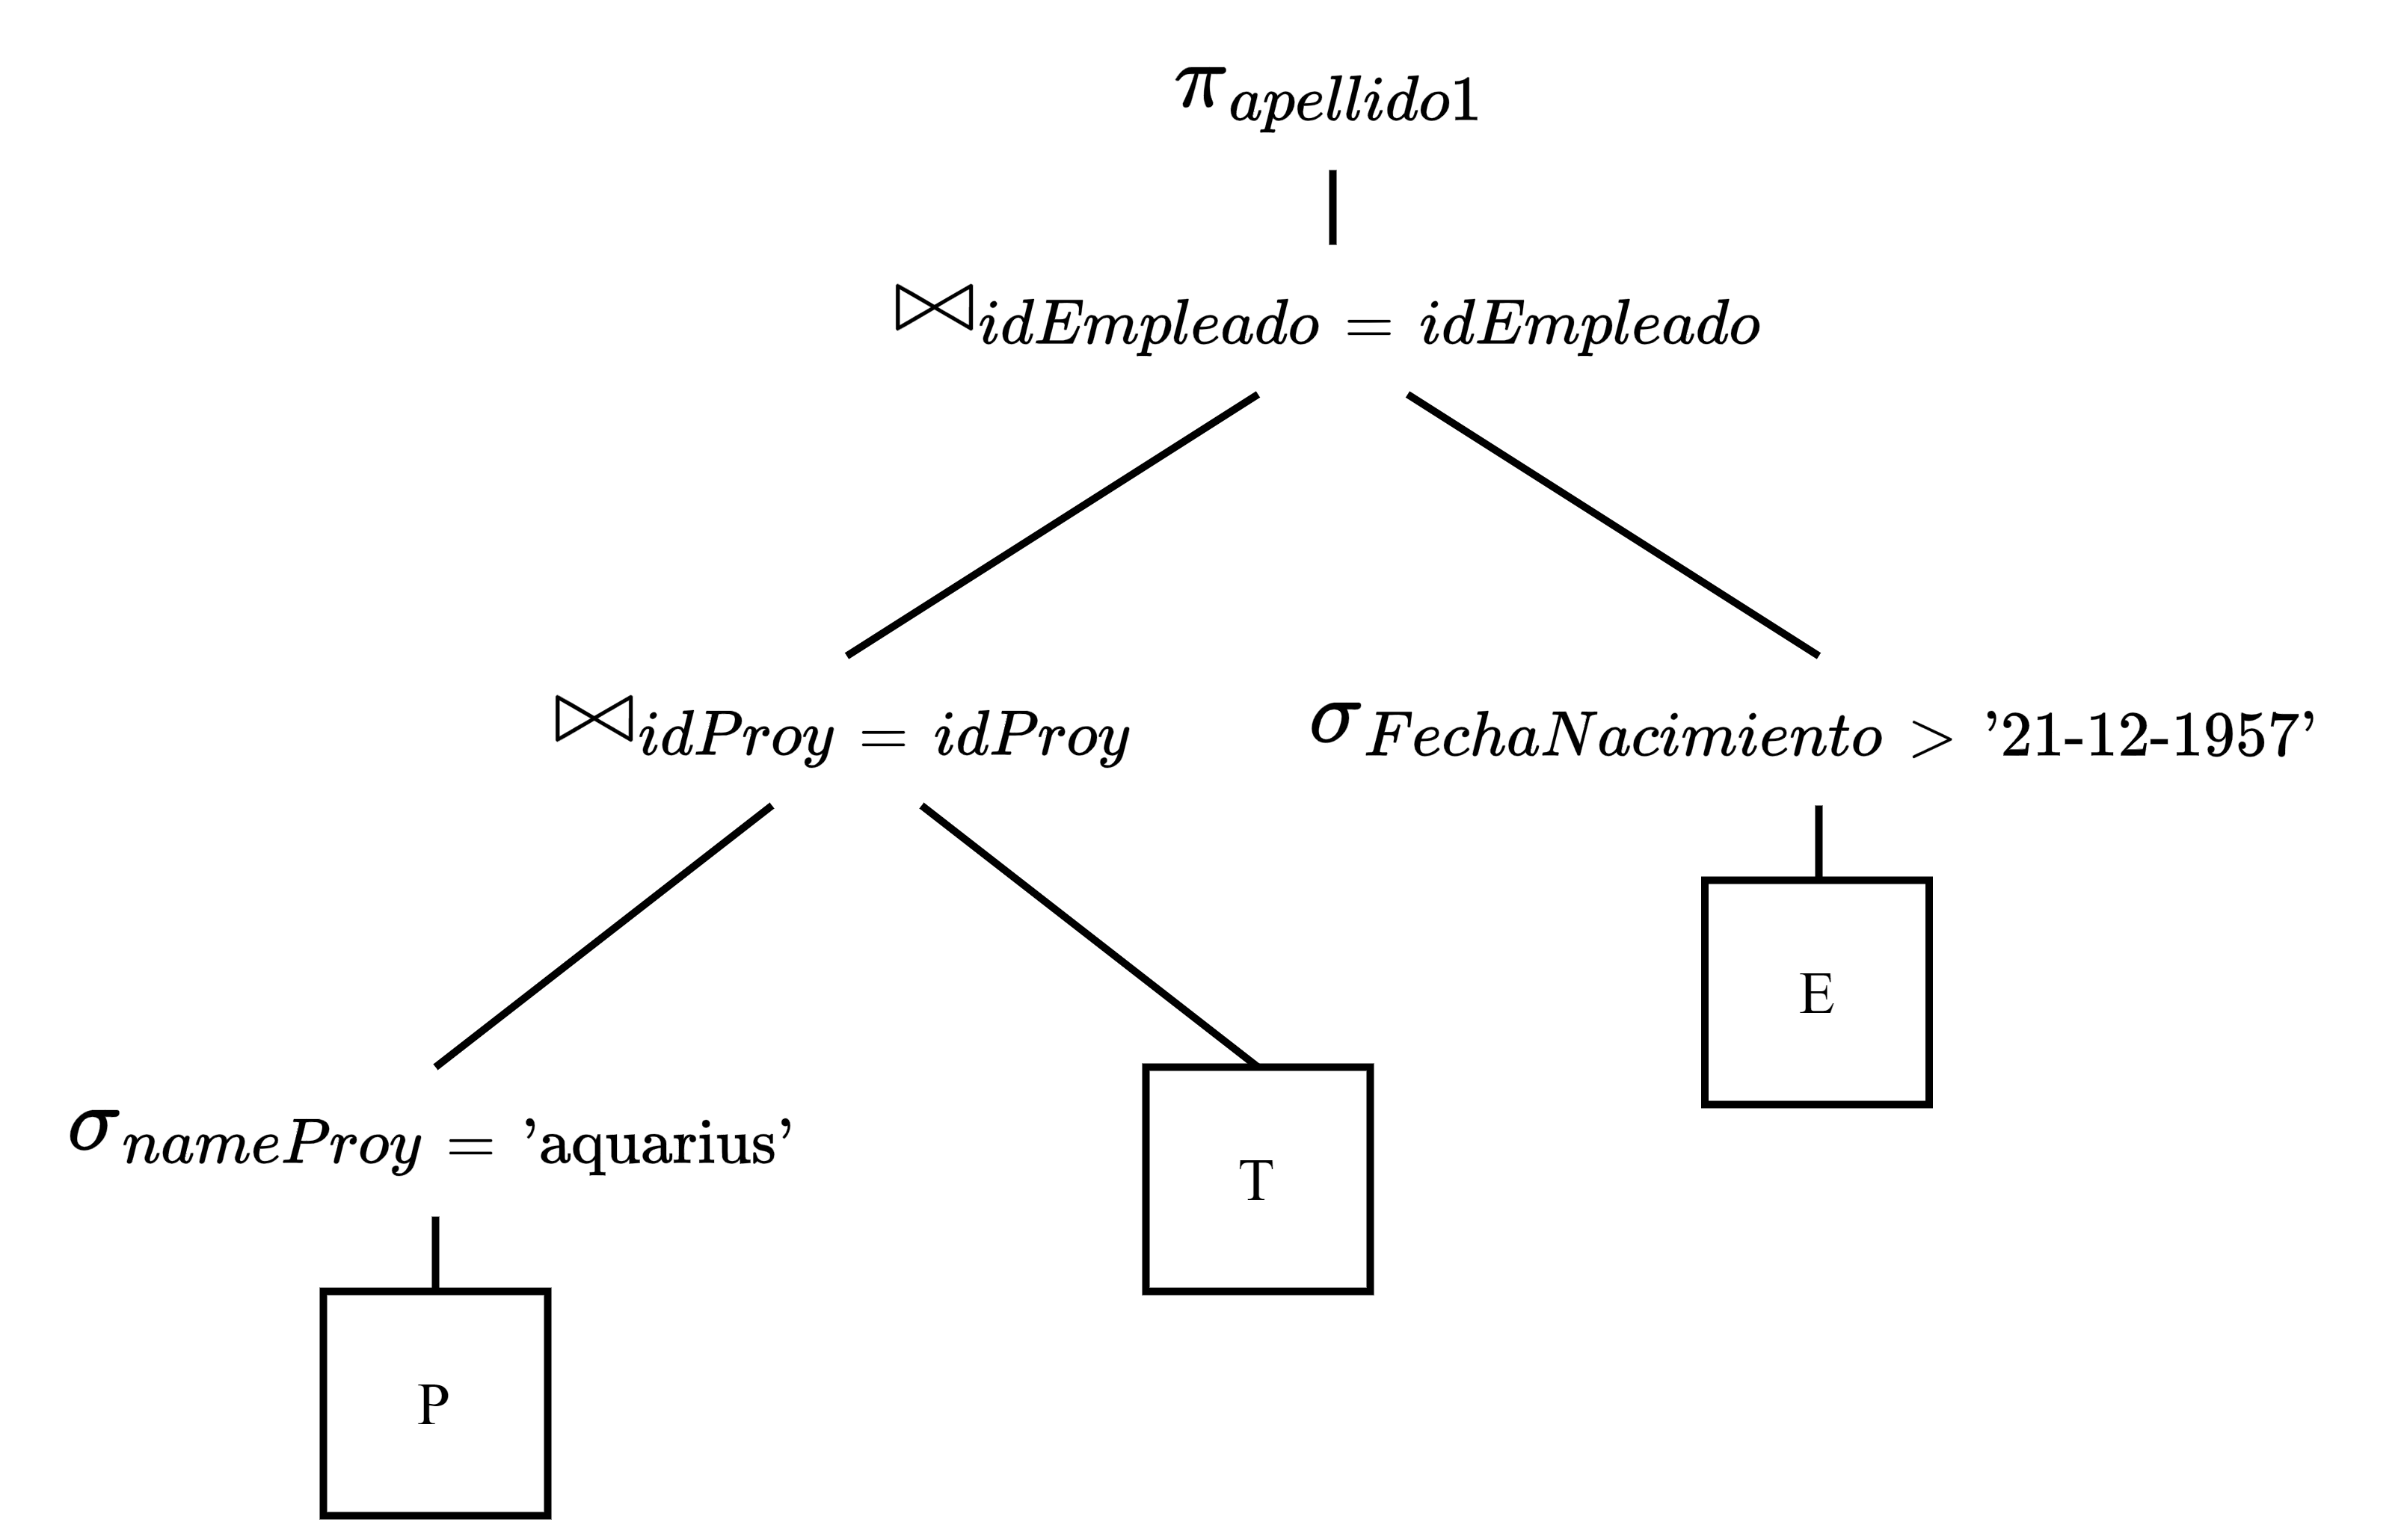
\includegraphics[width=0.8\textwidth]{img/E1-Paso5.png}
            \end{figure}

            \newpage
            \item Se proyecta solo lo necesario en las sub-tablas.
            \begin{figure}[H]
                \centering
                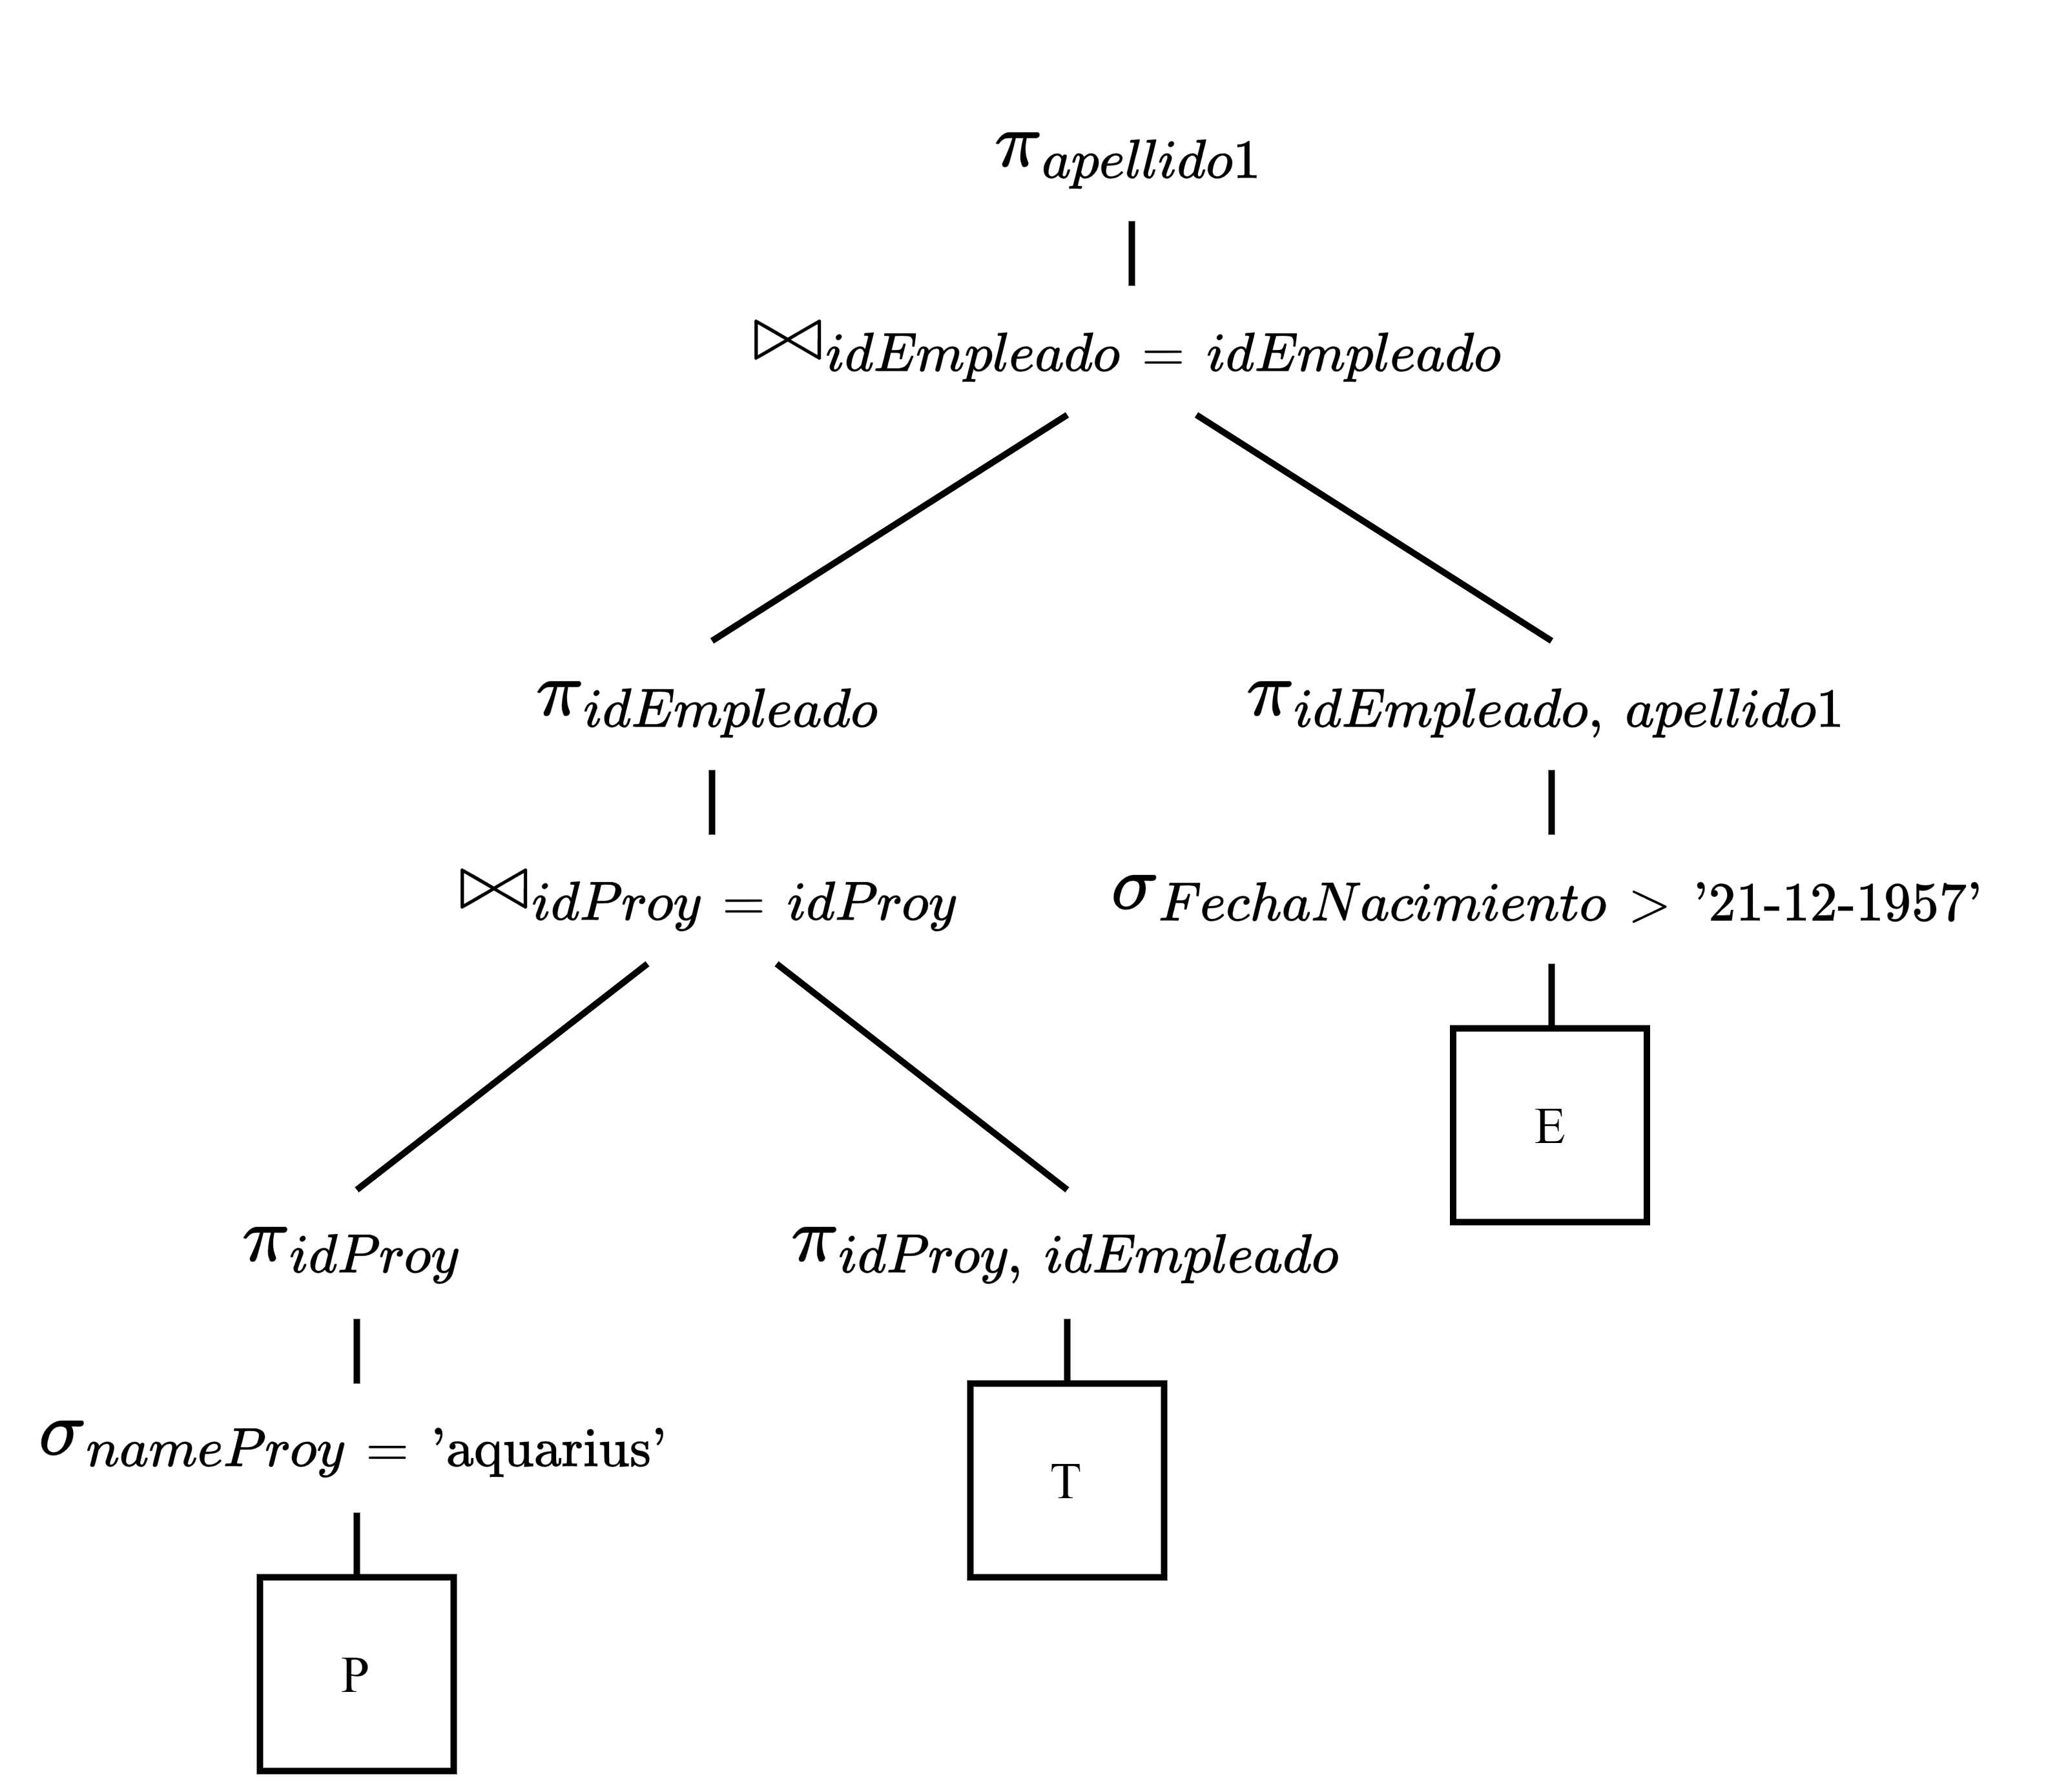
\includegraphics[width=\textwidth]{img/E1-Paso6.png}
            \end{figure}
        \end{enumerate}
    \end{enumerate}

    \newpage
    \item Considere las siguientes relaciones:
    \begin{itemize}
        \item \textbf{Variedades}(IdVar, Nombre, Prog2, Prog1)

        \item \textbf{Predios}(IdPredio, NombrePredio, Comuna, Superficie)

        \item \textbf{Siembra}(IdPredio, IdVar, HaSem, Rdto, añoA)
    \end{itemize}
    Sea la siguiente consulta: \newline
    \textit{"Listar los nombres de las variedades sembradas en el predio IdPredio = 10 y que el año 2015 tuvieron un rendimiento mayor a 60 qq/ha."}
    \begin{enumerate}
        \item Escriba la consulta SQL para la consulta anterior.
        \begin{tcolorbox}[
            colback=Verde!30,
            colframe=Verde!90!black]
            \begin{verbatim}
SELECT Nombre
FROM Variedades V, Siembra S
WHERE S.IdPredio = 10
AND V.IdVar = S.IdVar
AND S.añoA = 2015
AND S.Rdto > 60;
            \end{verbatim}
        \end{tcolorbox}
        \item Escriba la consulta en Algebra Relacional para la consulta anterior.
        \begin{align*}
            \scalebox{1.5}{$\pi$}_{\text{Nombre}} (
                \scalebox{1.5}{$\sigma$}_{
                    \scalebox{0.8}{
                        $\begin{array}{l}
                            \text{IdPredio} = 10 \; \wedge \\
                            \text{IdVar} = \text{IdVar} \; \wedge \\
                            \text{a\~noA} = 2015 \; \wedge \\
                            \text{Rdto} > 60
                        \end{array}$
                    }
                } (
                    \text{Variedades}_{\scalebox{1.3}{$\Join$}} \text{Siembra}
                )
            )
        \end{align*}

        \item Obtener el árbol inicial(canónico) de la consulta.
        \begin{figure}[H]
            \centering
            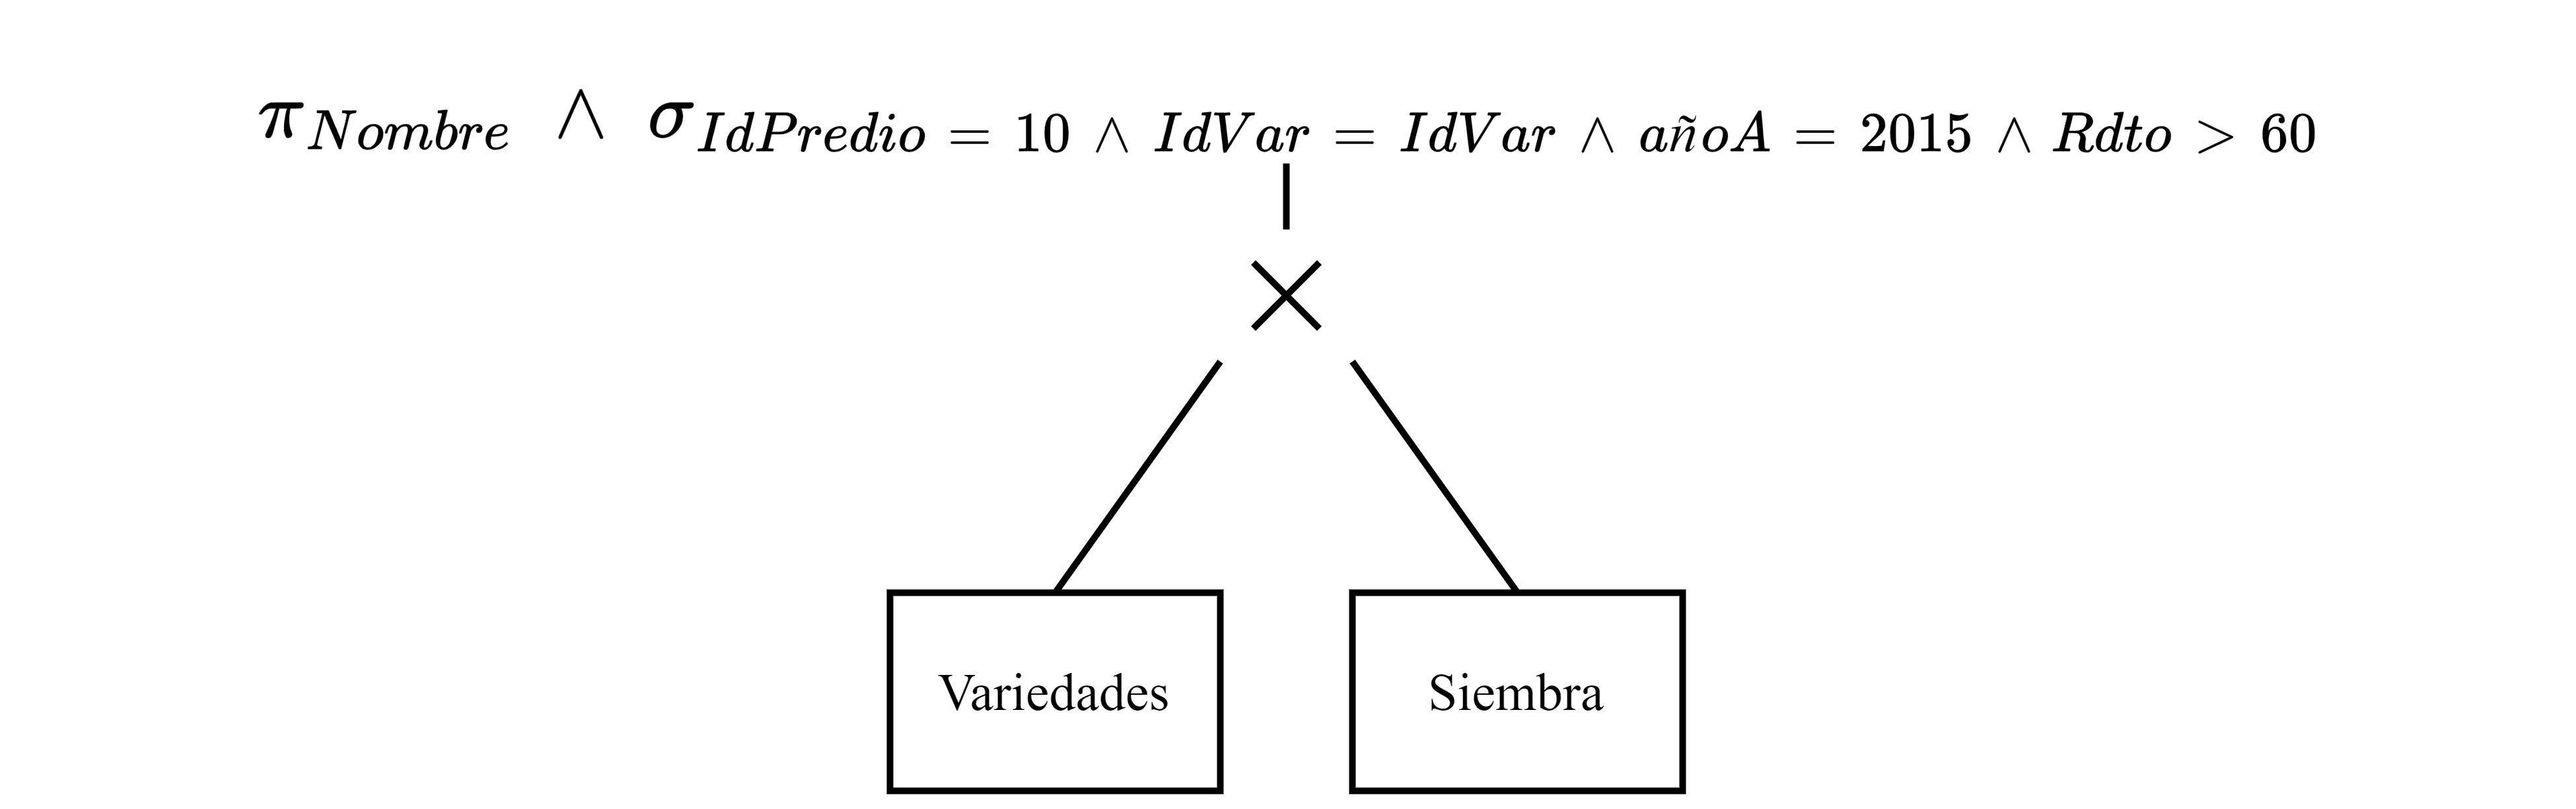
\includegraphics[width=\textwidth]{img/E2-ArbolCanonico.png}
        \end{figure}

        \newpage
        \item Explique como se optimiza el árbol de consulta mediante el algoritmo de optimización algebraica (visto en clases).
        \begin{enumerate}
            \item Se separa la proyección y las selecciones por tablas.
            \begin{figure}[H]
                \centering
                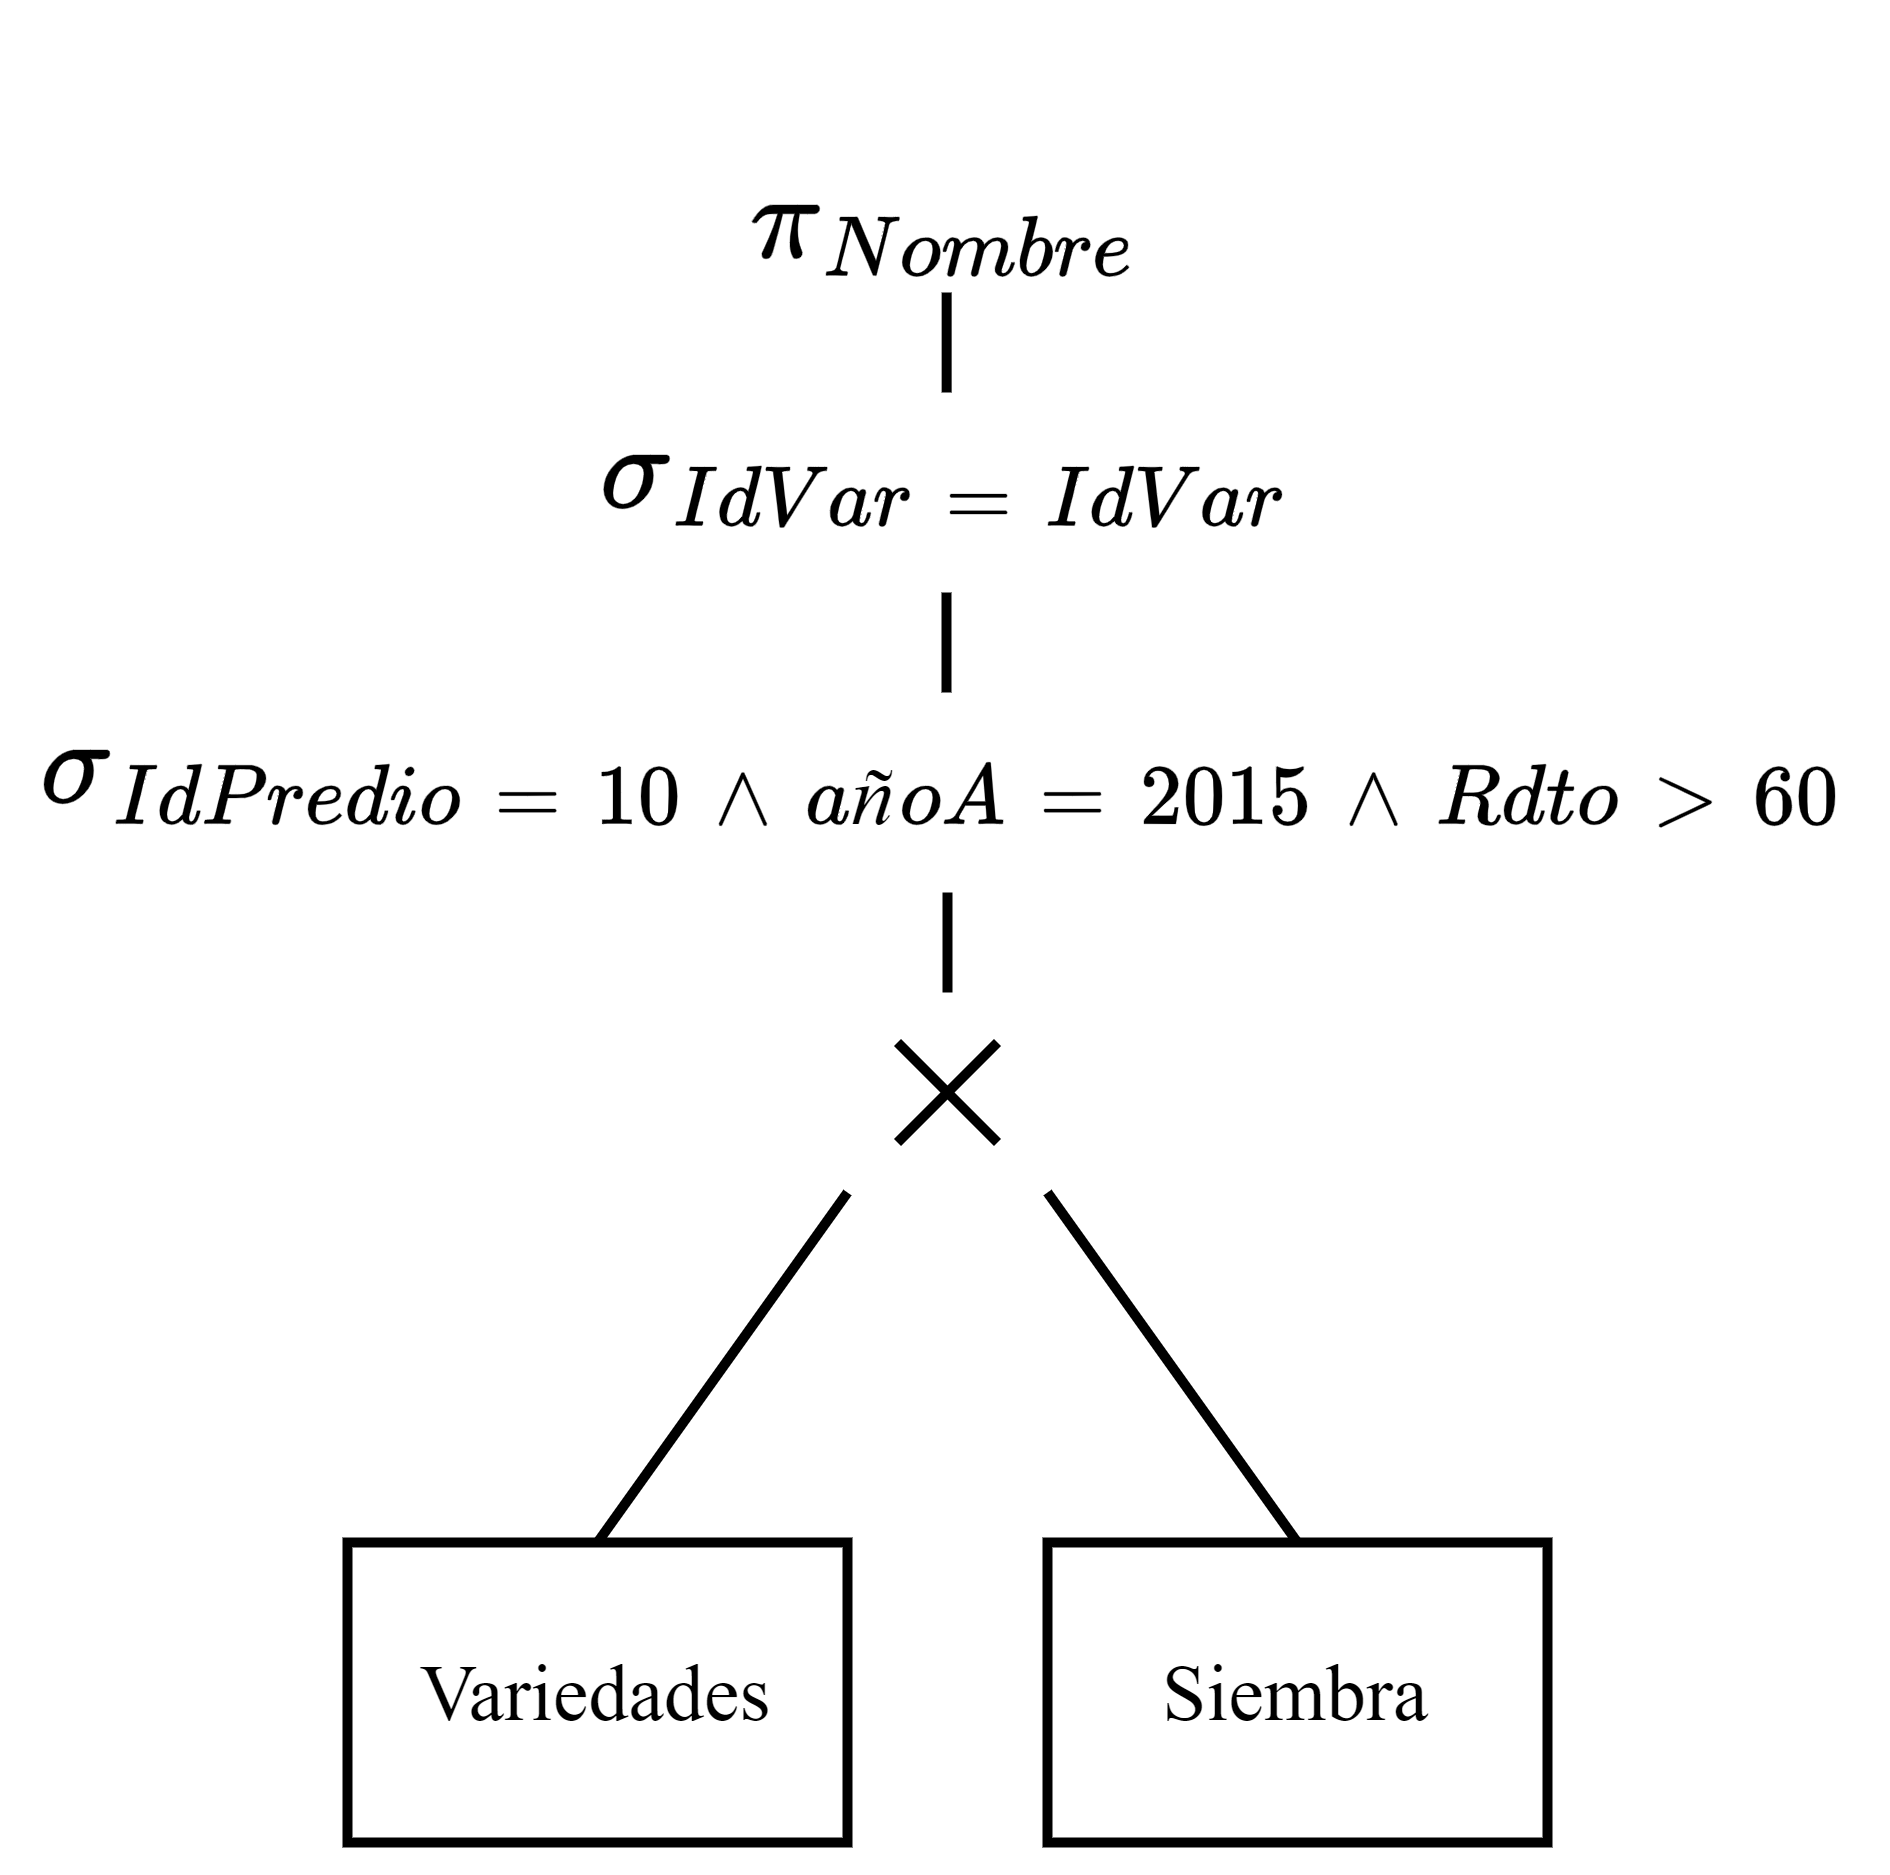
\includegraphics[width=0.6\textwidth]{img/E2-Paso1.png}
            \end{figure}

            \item Se reorganizan las tablas buscando la forma más optimas de unir las tablas (Solo si es posible).

            \item Se bajan las selecciones hasta su respectivo producto cartesiano.
            \begin{figure}[H]
                \centering
                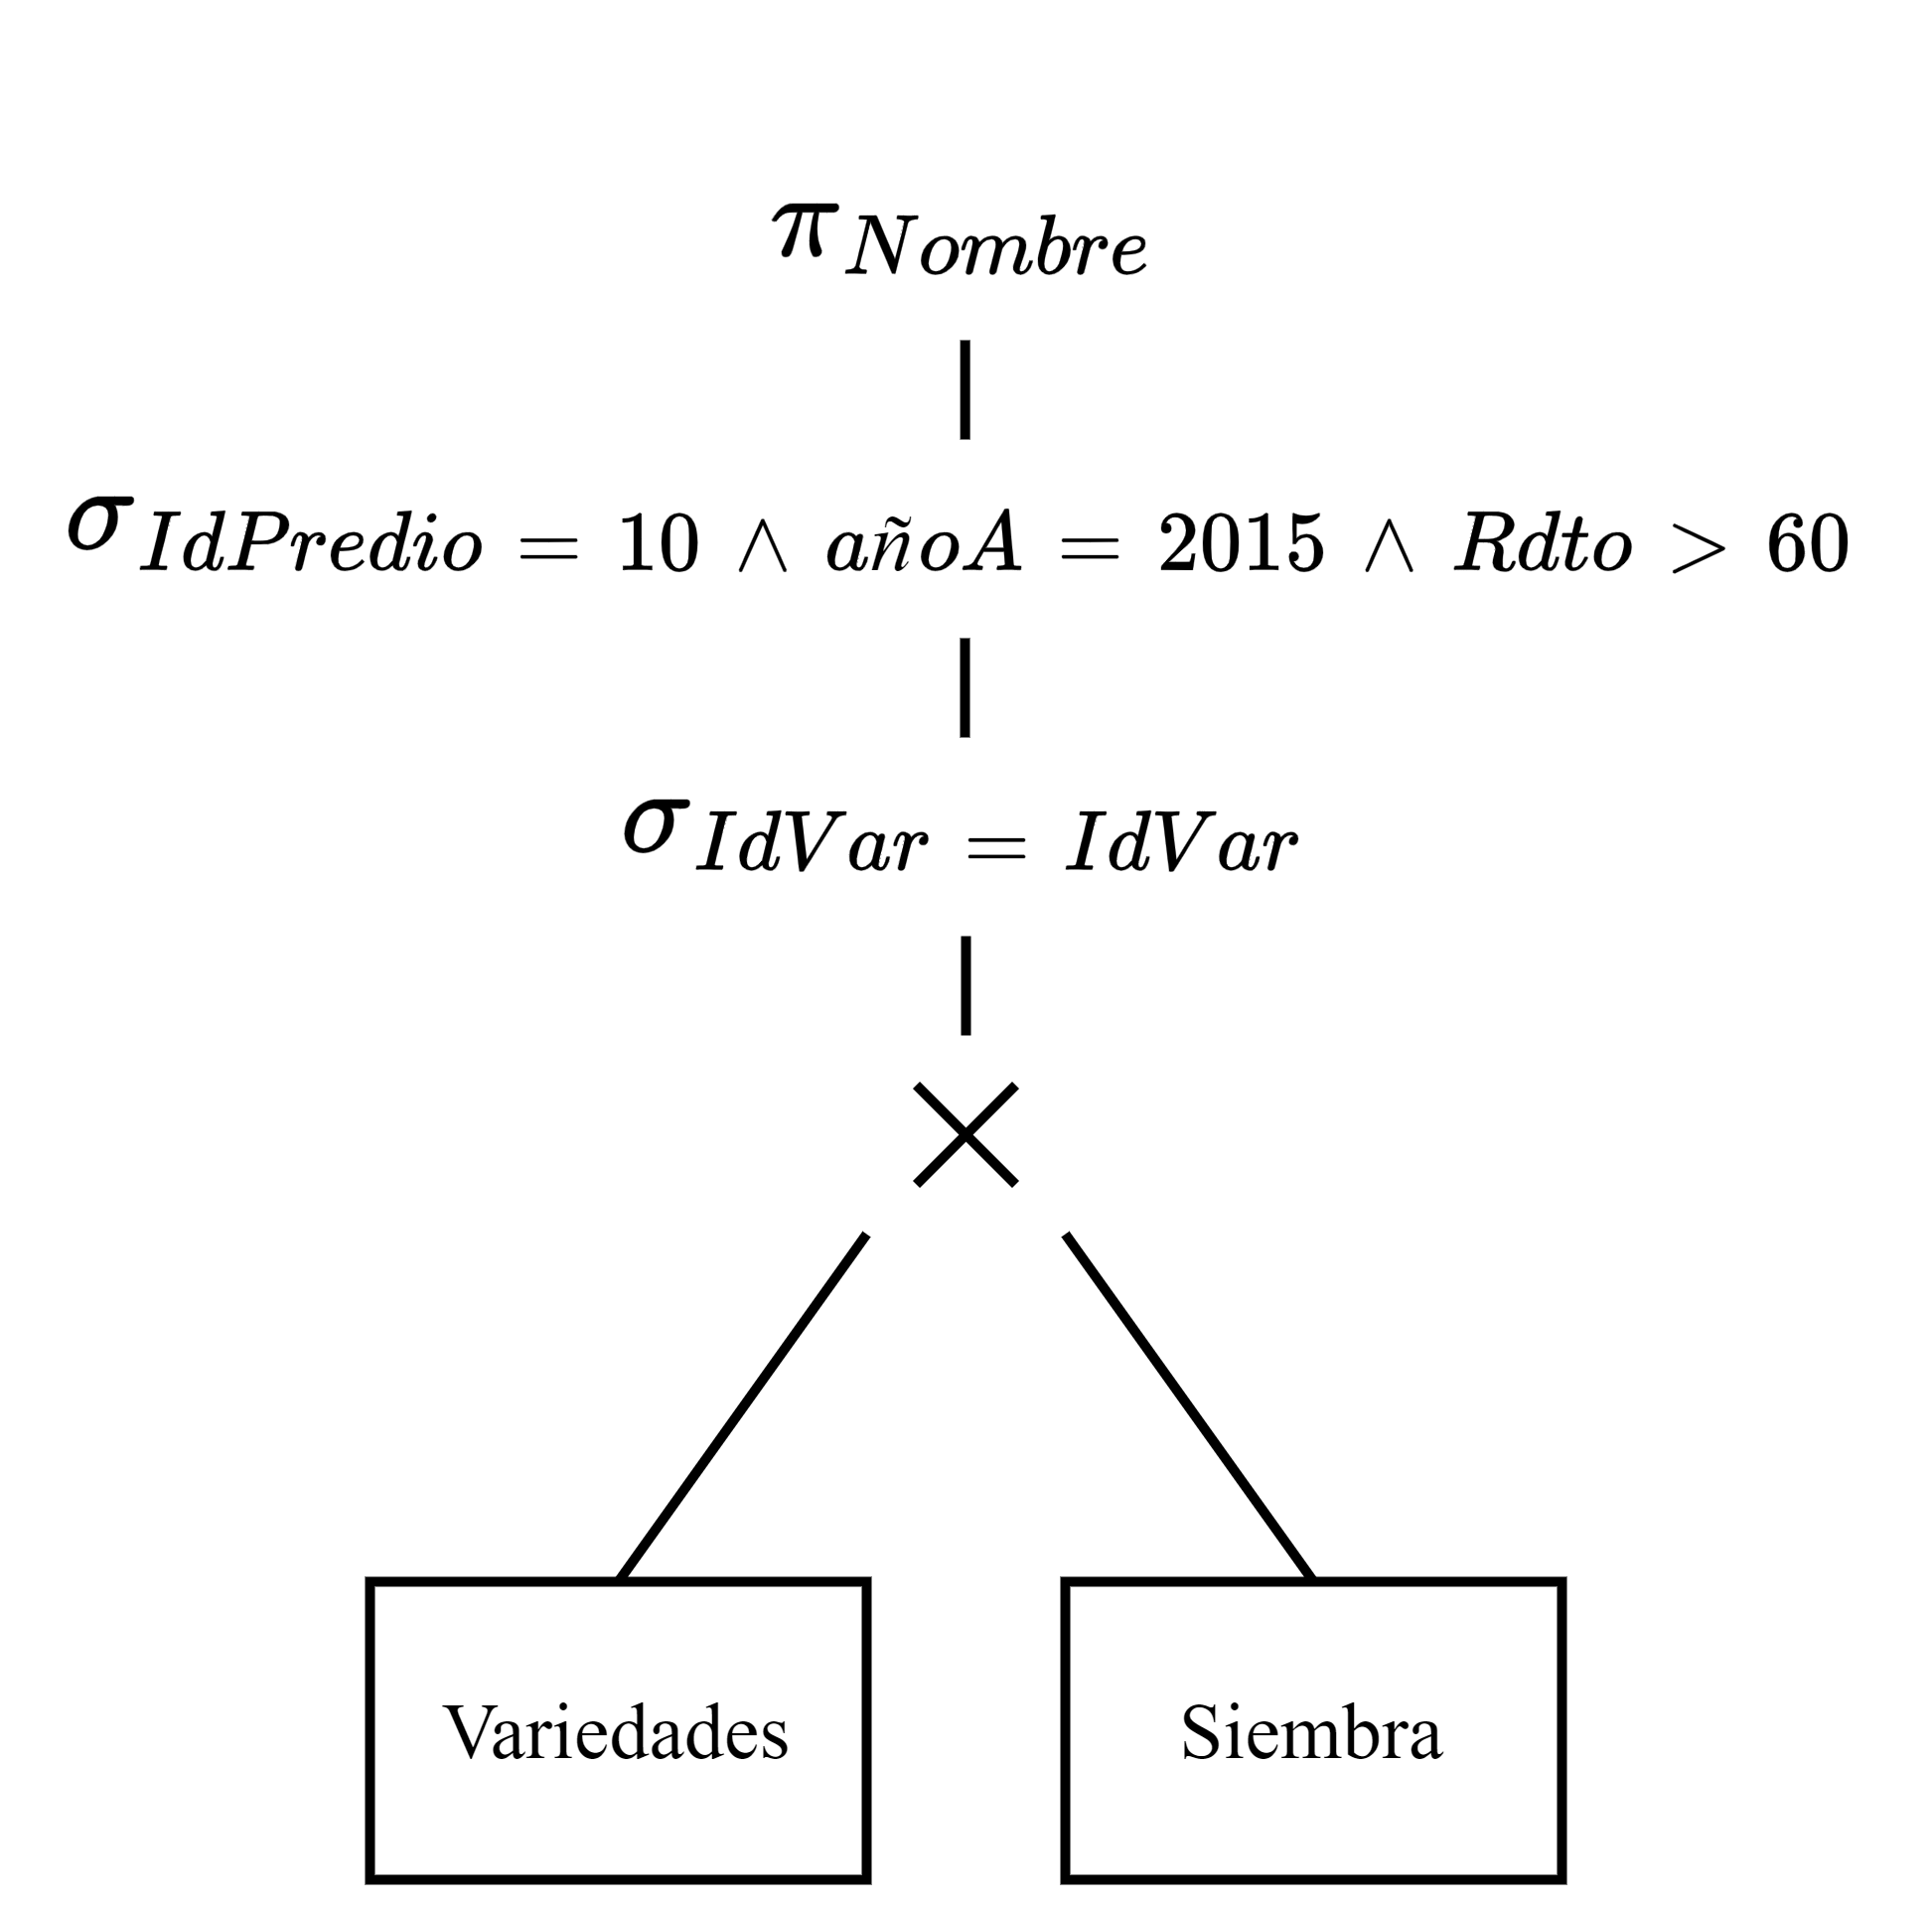
\includegraphics[width=0.6\textwidth]{img/E2-Paso3.png}
            \end{figure}

            \newpage
            \item Se cambia la seleccion y el producto cartesiano por un join.
            \begin{figure}[H]
                \centering
                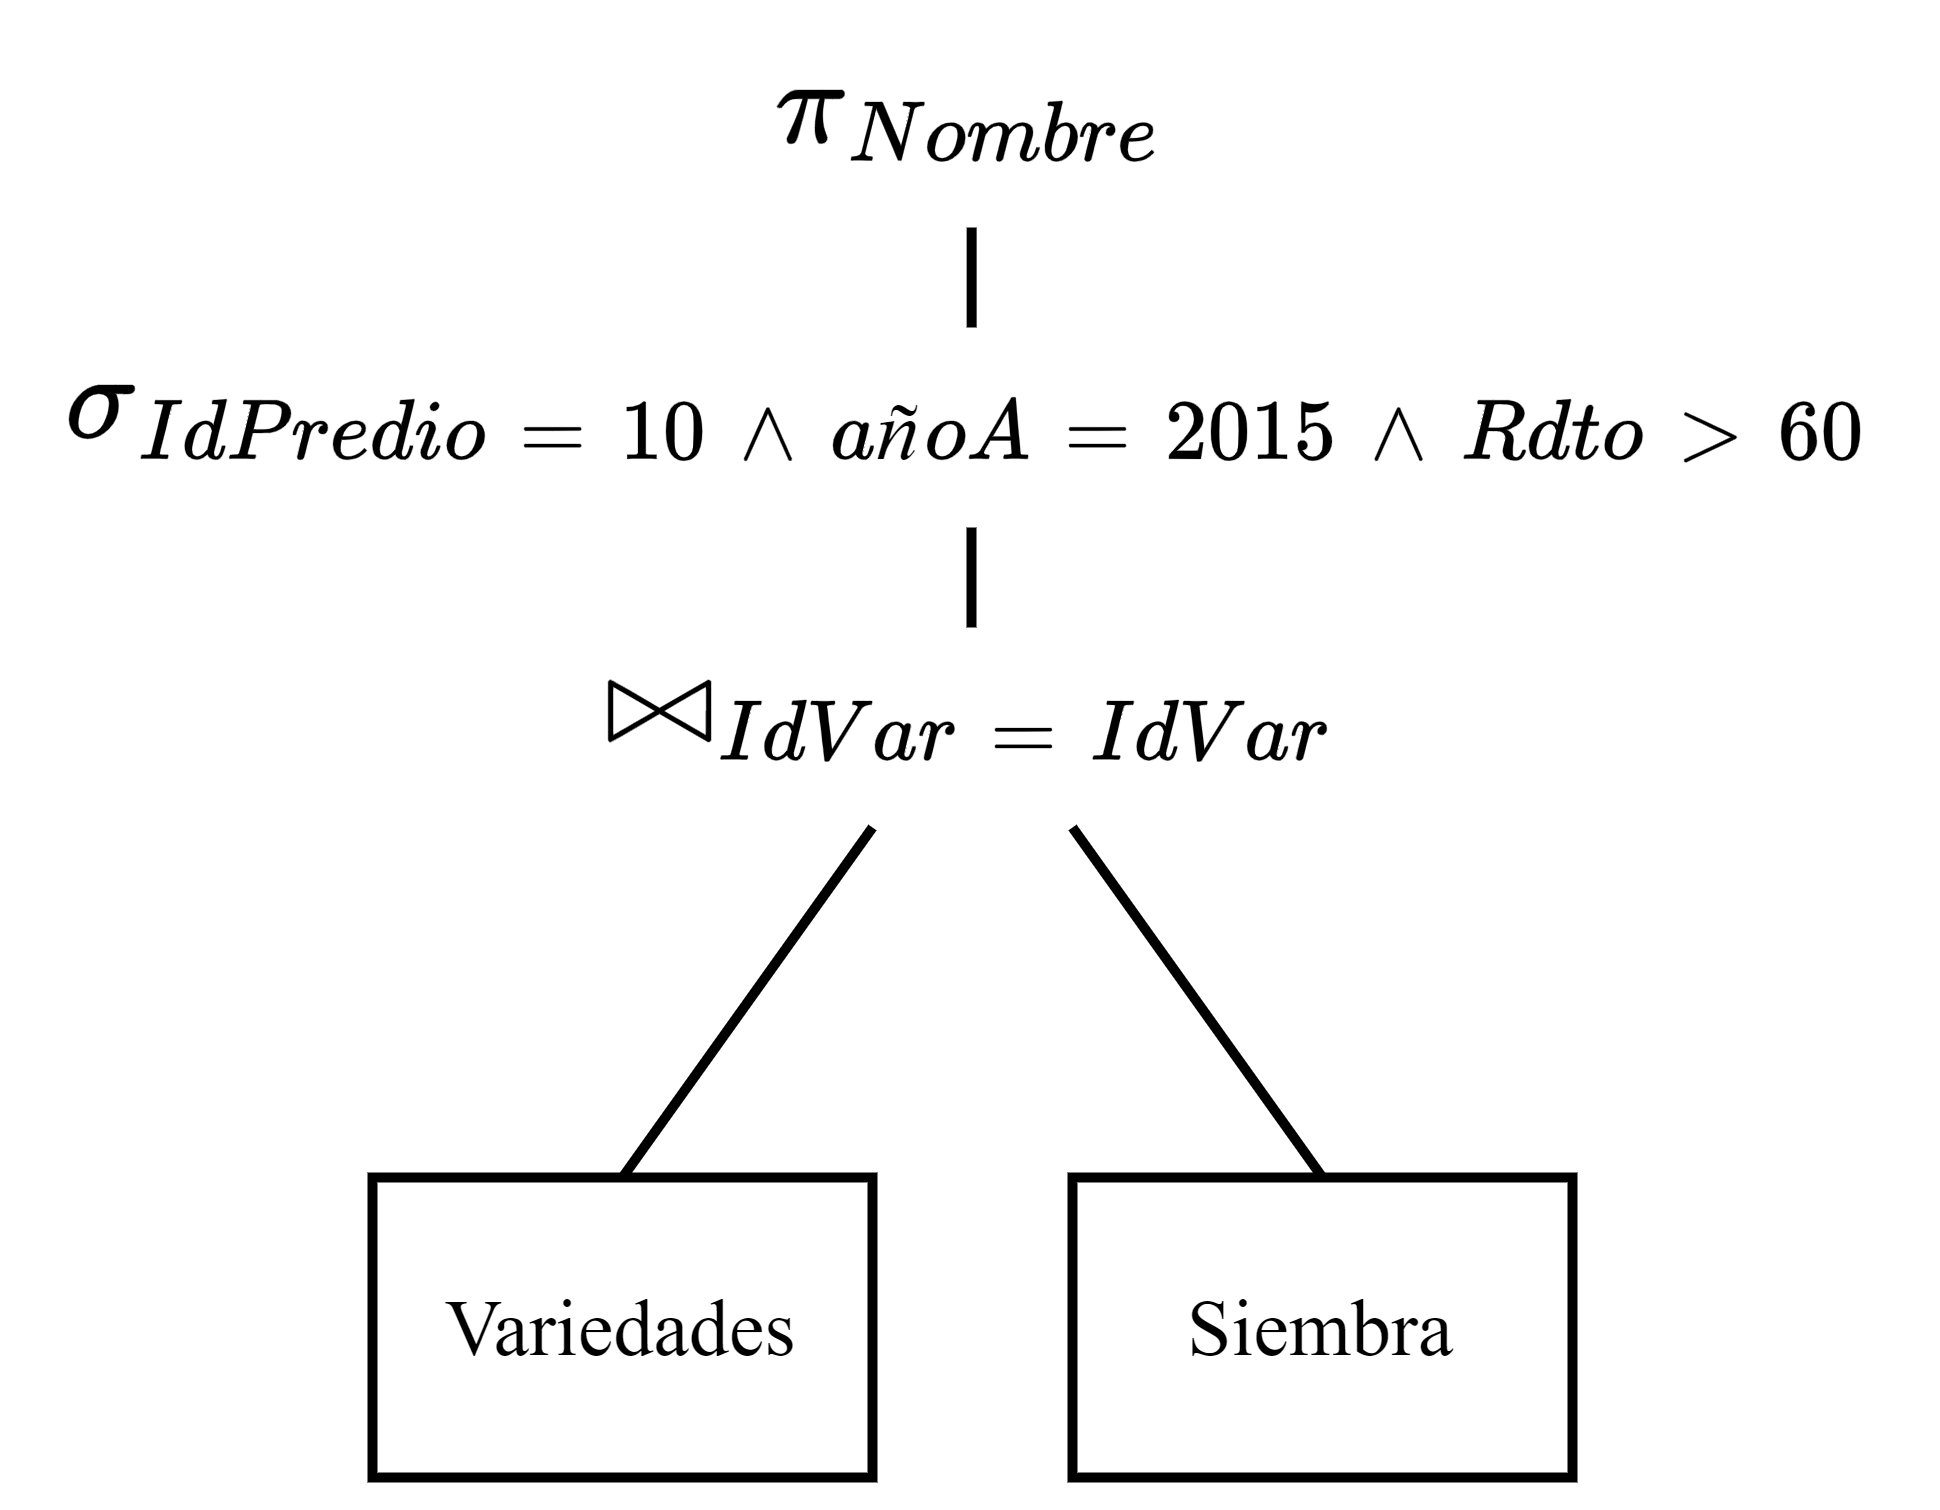
\includegraphics[width=0.5\textwidth]{img/E2-Paso4.png}
            \end{figure}

            \item Se bajan las demas selecciones a sus respectivas tablas.
            \begin{figure}[H]
                \centering
                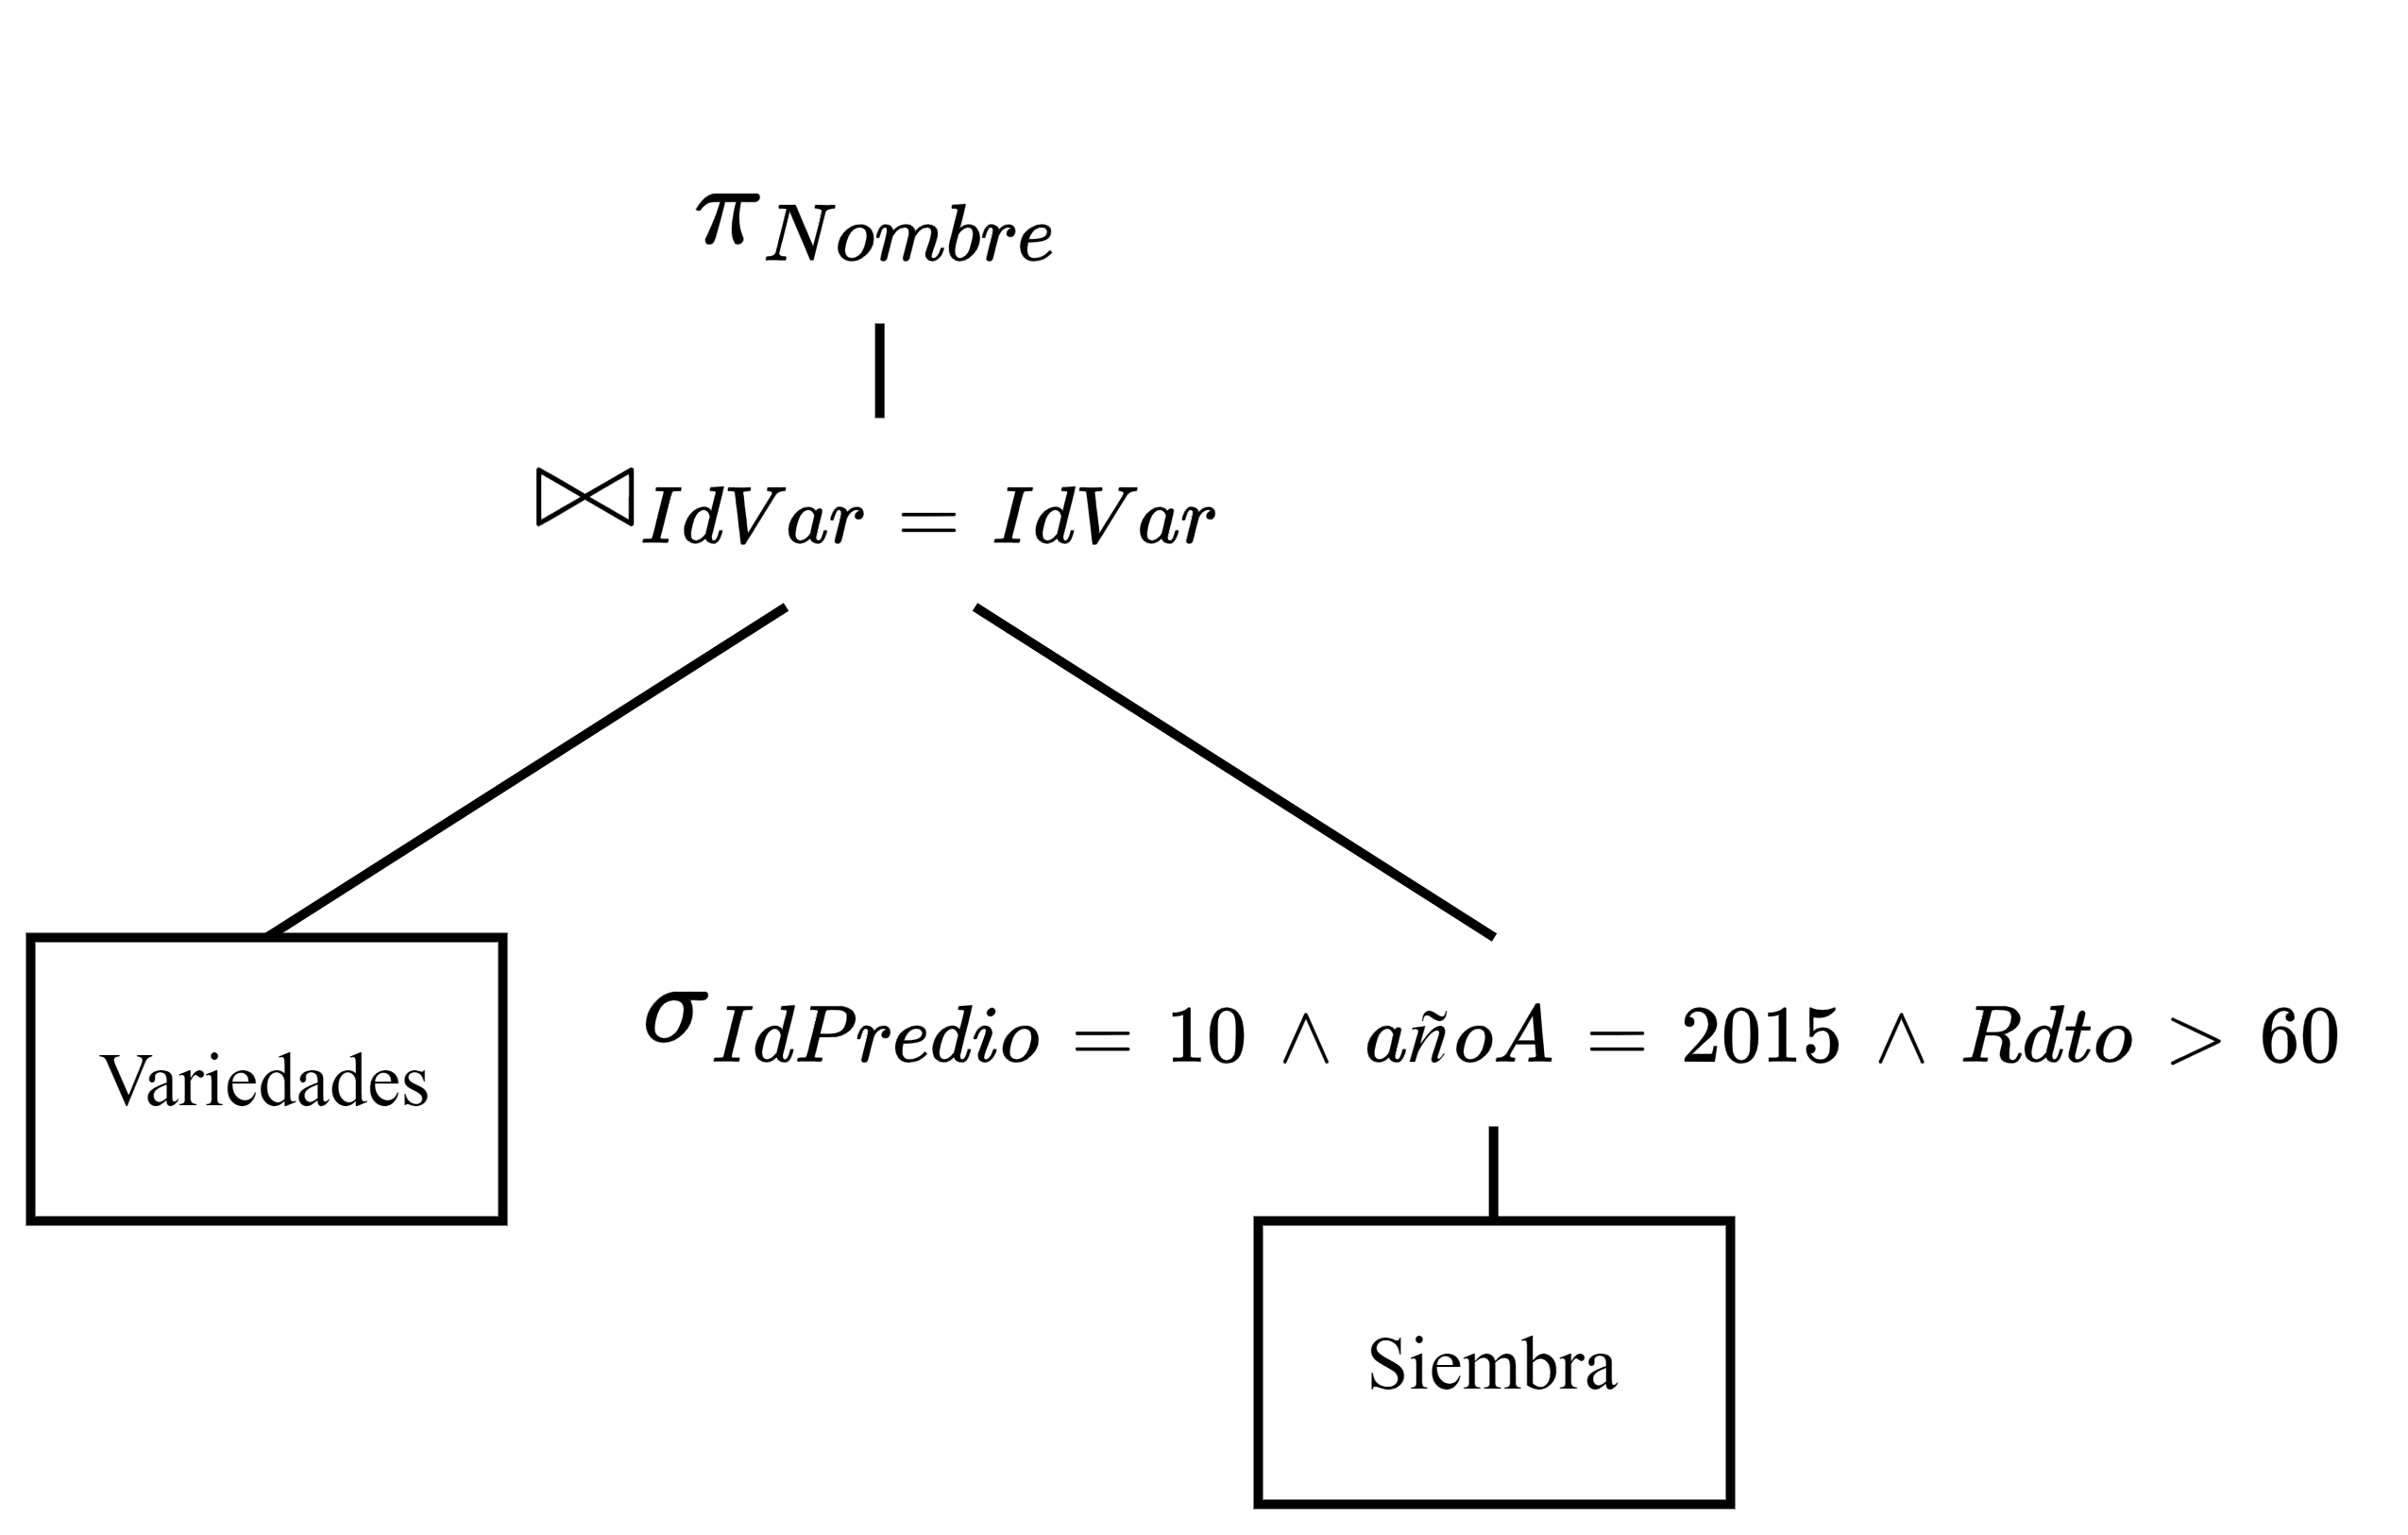
\includegraphics[width=0.6\textwidth]{img/E2-Paso5.png}
            \end{figure}

            \item Se proyecta solo lo necesario en las sub-tablas.
            \begin{figure}[H]
                \centering
                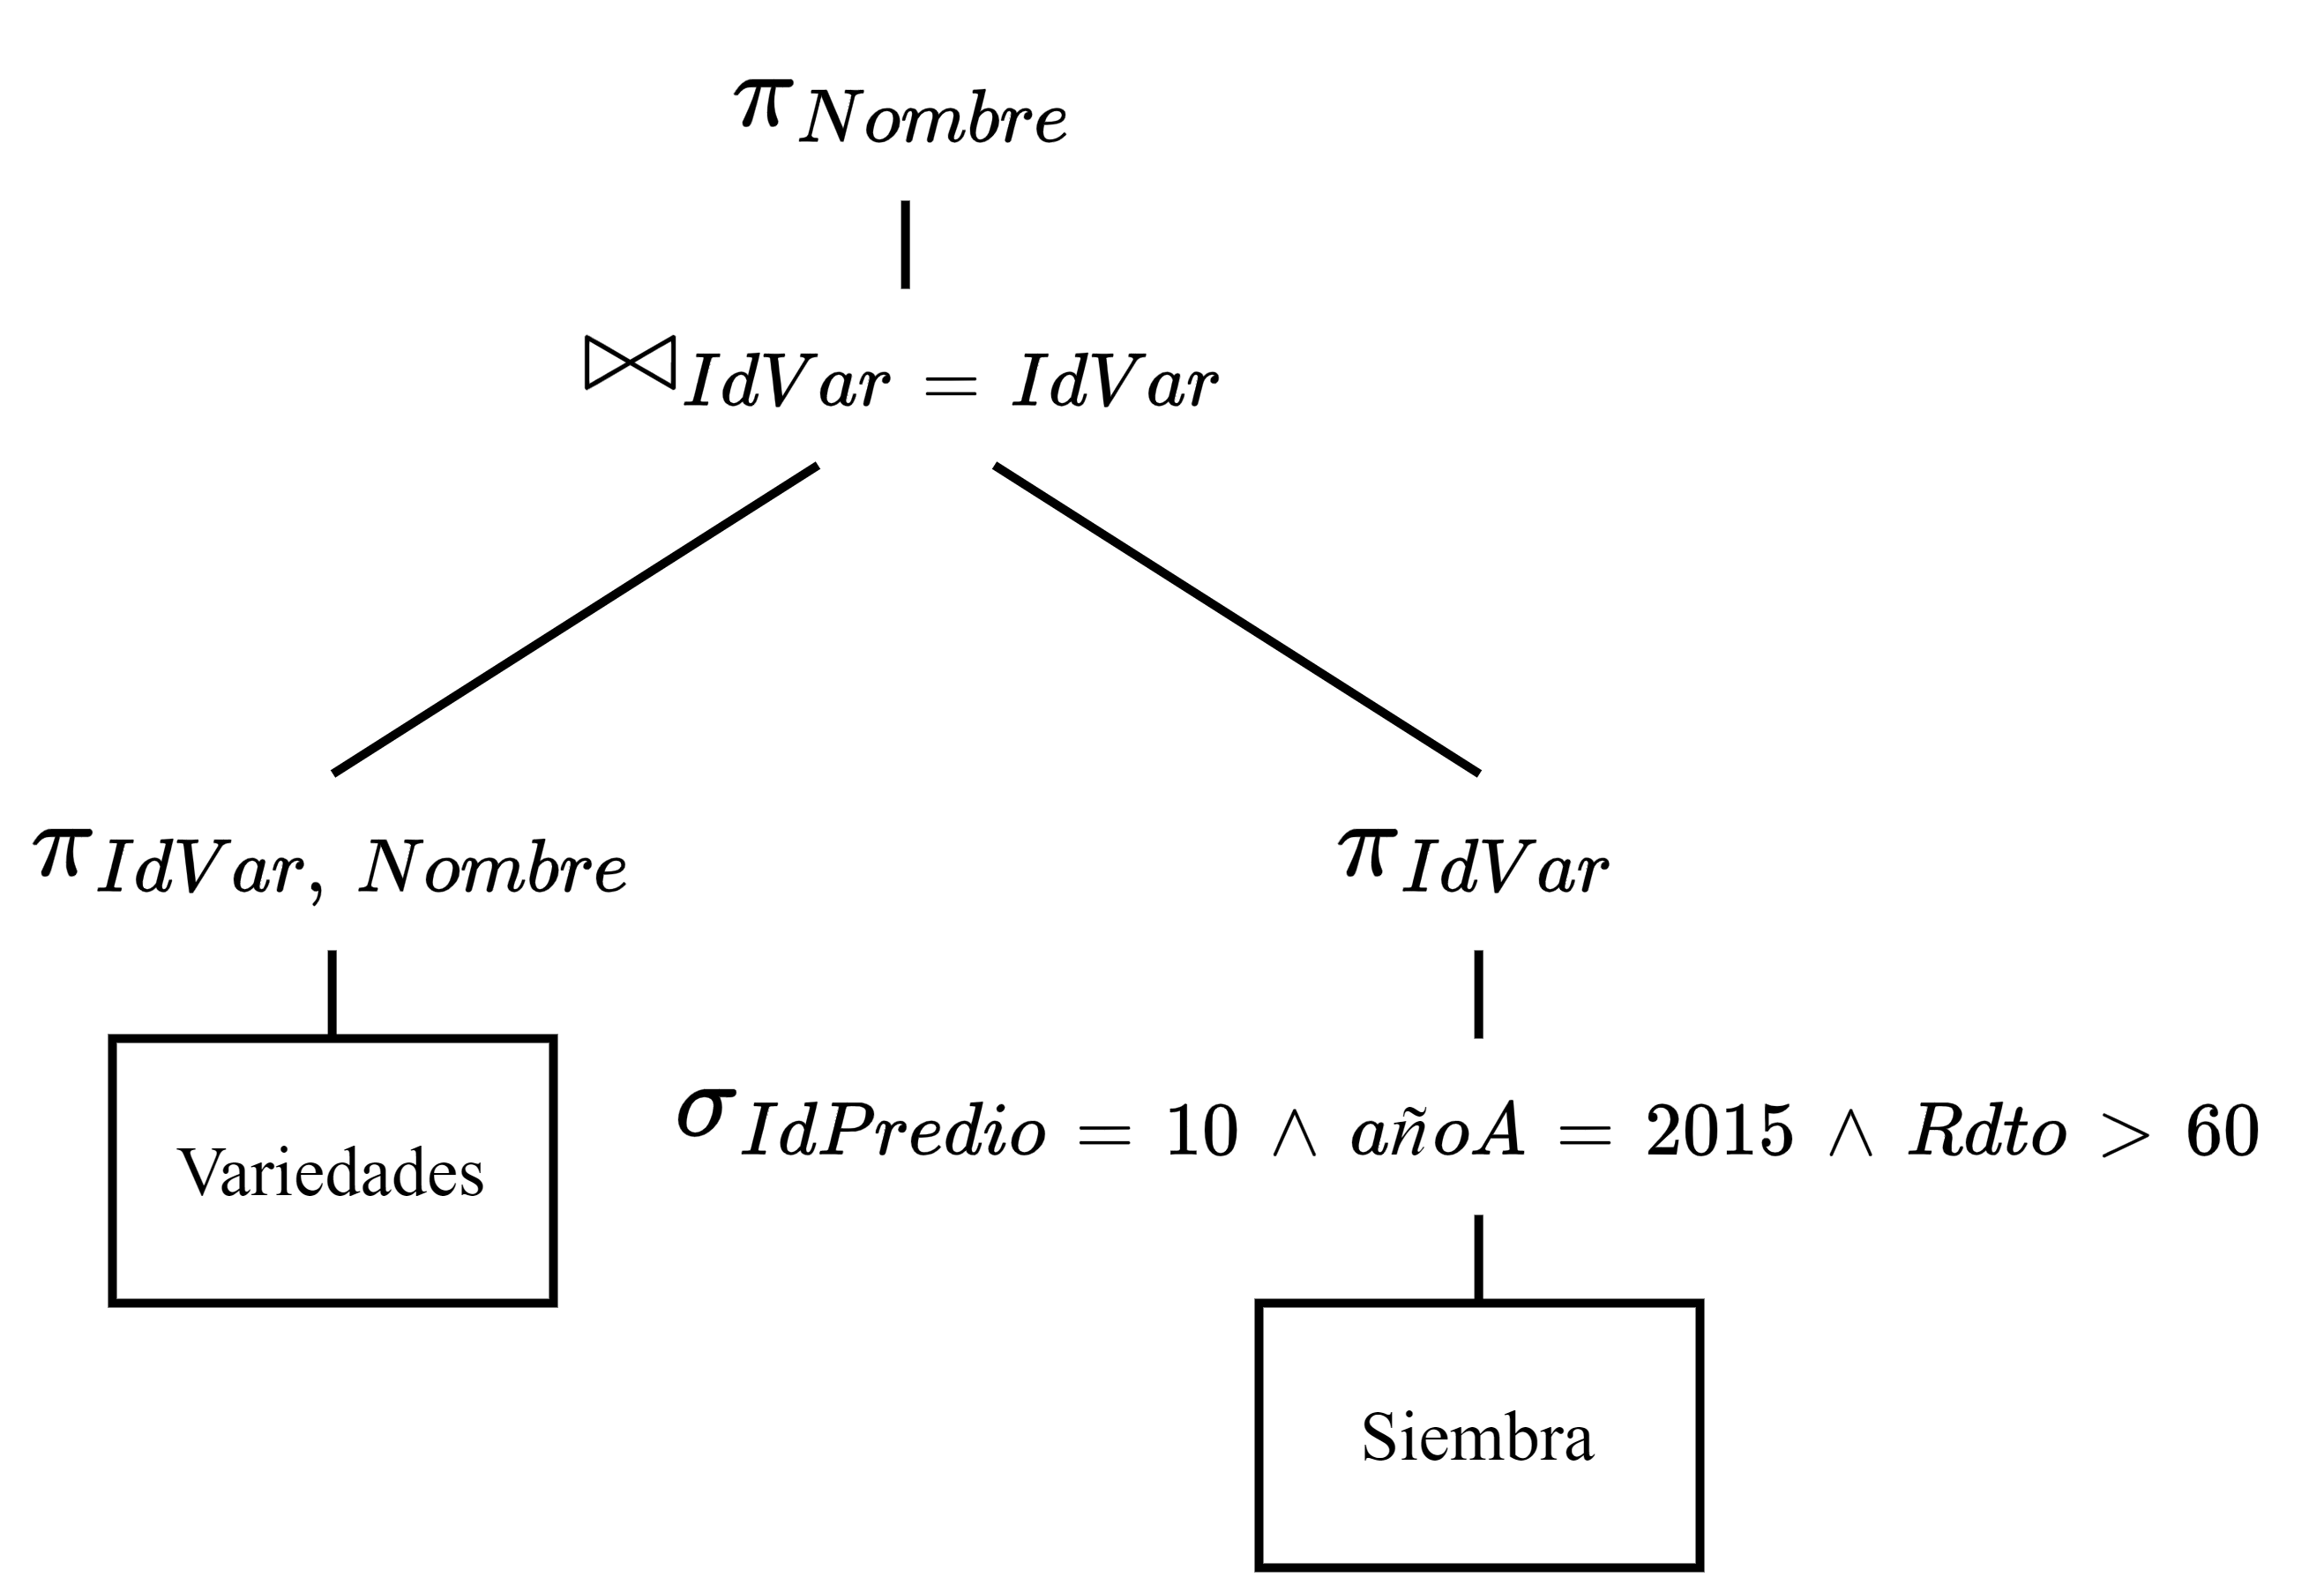
\includegraphics[width=0.6\textwidth]{img/E2-Paso6.png}
            \end{figure}
        \end{enumerate}
    \end{enumerate}

    \newpage
    \textbf{Para 3 y 4, calcular un orden/JOINS para R, S, T, U, usando programación dinámica (como visto en clases). Mostrar tabla inicial de costos, los calculos de cada etapa y árboles.}
    \item Suponer que tenemos las relaciones R(a, b), S(b, c), T(c, d) y U(d, e) con las siguientes características:
    \newparagraph
    \begin{minipage}{0.5\textwidth}
        \begin{itemize}
            \item T(R) = 300
            \item V(R, b) = 100
            \item T(S) = 200
            \item V(S, b) = 100
            \item V(S, c) = 20
        \end{itemize}
    \end{minipage}
    \hfill
    \begin{minipage}{0.5\textwidth}
        \begin{itemize}
            \item T(T) = 150
            \item V(T, c) = 20
            \item V(T, d) = 300
            \item T(U) = 500
            \item V(U, d) = 300
        \end{itemize}
    \end{minipage}

    \newpage
    \item Suponer que tenemos las relaciones R(a, b), S(b, c), T(c, d) y U(d, e) con las siguientes características:
    \newparagraph
    \begin{minipage}{0.5\textwidth}
        \begin{itemize}
            \item T(R) = 50
            \item V(R, b) = 250
            \item T(S) = 55
            \item V(S, b) = 500
            \item V(S, c) = 5
        \end{itemize}
    \end{minipage}
    \hfill
    \begin{minipage}{0.5\textwidth}
        \begin{itemize}
            \item T(T) = 50
            \item V(T, c) = 15
            \item V(T, d) = 500
            \item T(U) = 45
            \item V(U, d) = 50
        \end{itemize}
    \end{minipage}
\end{enumerate}
\end{document}